\documentclass[11pt,a4paper]{article}

\usepackage[utf8]{inputenc}
\usepackage[T1]{fontenc}
\usepackage{lmodern}
\usepackage[a4paper,margin=2.5cm]{geometry}
\usepackage{graphicx}
\usepackage{booktabs}
\usepackage{longtable}
\usepackage{array}
\usepackage{amsmath,amssymb}
\usepackage{xcolor}
\usepackage{listings}
\usepackage{tikz}
\usetikzlibrary{arrows.meta,positioning,shapes.geometric}
\usepackage{fancyhdr}
\usepackage{float}
\usepackage{caption}
\usepackage{enumitem}
\usepackage{microtype}
\usepackage[colorlinks=true,linkcolor=blue!50!black,urlcolor=blue!50!black,citecolor=blue!50!black]{hyperref}
\usepackage[most]{tcolorbox}


\usepackage{tabularx}
\usepackage{booktabs}
\usepackage{float}



\setlength{\headheight}{14pt}
\setlength{\emergencystretch}{3em}
\renewcommand{\_}{\textunderscore\allowbreak{}}
\setlength{\parskip}{0.5em}
\setlength{\parindent}{0pt}
\renewcommand{\arraystretch}{1.15}

\pagestyle{fancy}
\fancyhf{}
\lhead{RAG for Image Captioning on MS COCO}
\rhead{Data exploration and pre-processing}
\cfoot{\thepage}

\lstset{
  basicstyle=\ttfamily\footnotesize,
  breaklines=true,
  frame=single,
  backgroundcolor=\color{gray!6},
  rulecolor=\color{gray!50},
  columns=fullflexible,
  keepspaces=true
}

\newtcolorbox{interp}[1][Interpretation]{
  colback=blue!4, colframe=blue!50!black, fonttitle=\bfseries\small,
  title=#1, boxrule=0.6pt, arc=2pt, left=6pt, right=6pt, top=4pt, bottom=4pt
}
\newtcolorbox{remark}[1][Remark]{
  colback=orange!6, colframe=orange!70!black, fonttitle=\bfseries\small,
  title=#1, boxrule=0.6pt, arc=2pt, left=6pt, right=6pt, top=4pt, bottom=4pt
}

\newcommand{\code}[1]{\texttt{#1}}

\begin{document}

%====================================================================
\begin{titlepage}
\centering
\vspace*{2cm}
{\Large Image Processing Mini-Project}\\[1.2cm]
{\LARGE\bfseries A Comparative Study of RAG Techniques\\[0.3cm] for Generating Image Captions}\\[1.5cm]
{\Large Phase 1 --- Data Exploration and Pre-processing}\\[0.8cm]
{\large Technical report}\\[2.5cm]


{\large Prepared by:}\\[0.8cm]

\begin{tabular}{c@{\hspace{4cm}}c}
Meradi Serine Feriel & Seba Bouchra \\[0.8cm]
Aggoune Abderrahim & Souchane Serine
\end{tabular}
\vfill
{\large Academic Year: 2026/2027}
\end{titlepage}

\tableofcontents
\newpage

%====================================================================
\section{Introduction and objectives of the phase}

Automatic image captioning is a core task at the crossroads of computer vision and natural language processing. Modern Vision--Language Models (VLMs) generate fluent captions, but they may \emph{omit} objects that are present, \emph{invent} objects that are absent (hallucination), or lack precision about attributes and relations. Retrieval-Augmented Generation (RAG) grounds the generation process in external evidence (similar images, reference captions, metadata), with the goal of improving accuracy, relevance and visual grounding~\cite{rag}.

The overall mini-project compares ten RAG techniques (naive/dense, sparse BM25, hybrid, reranking, multimodal, contextual compression, Self-RAG, corrective RAG, query expansion and metadata-filtered RAG) on a subset of MS COCO~\cite{coco}. The purpose of this first phase is therefore to transform the raw COCO data into a \emph{clean, reproducible and frozen} set of artefacts.

This report documents, step by step and in the order imposed by the project statement (Sections~4.3 and 4.4):
\begin{enumerate}[nosep]
  \item the \textbf{statistical exploration} of the dataset (object classes, scene complexity, textual statistics, diversity, visualisations);
  \item the \textbf{eight pre-processing steps} (plus the optional YOLO detection branch added to Step~5 and the extension of the test set to 1\,000 images): (1) data audit and validation, (2) split creation and anti-leakage control, (3) image pre-processing, (4) caption pre-processing, (5) metadata extraction, (6) embedding generation, (7) knowledge-base construction, (8) quality control;
  \item the \textbf{validation and freezing} of the release.
\end{enumerate}
For every step we describe the working method (script, algorithm, parameters), report the results obtained from the code outputs and generated files, and interpret them.






%====================================================================

\section{Project organisation and reproducibility}

\subsection{Pipeline overview}

The Data Preparation and Knowledge Base Construction Pipeline is implemented using a set of independent Python scripts, each responsible for a specific task. These scripts process the dataset through a series of stages, generating intermediate outputs and artefacts required by subsequent steps. Figure~\ref{fig:pipeline} summarises the flow of data.
\\
\begin{figure}[!htbp]
\centering
\resizebox{\textwidth}{!}{%
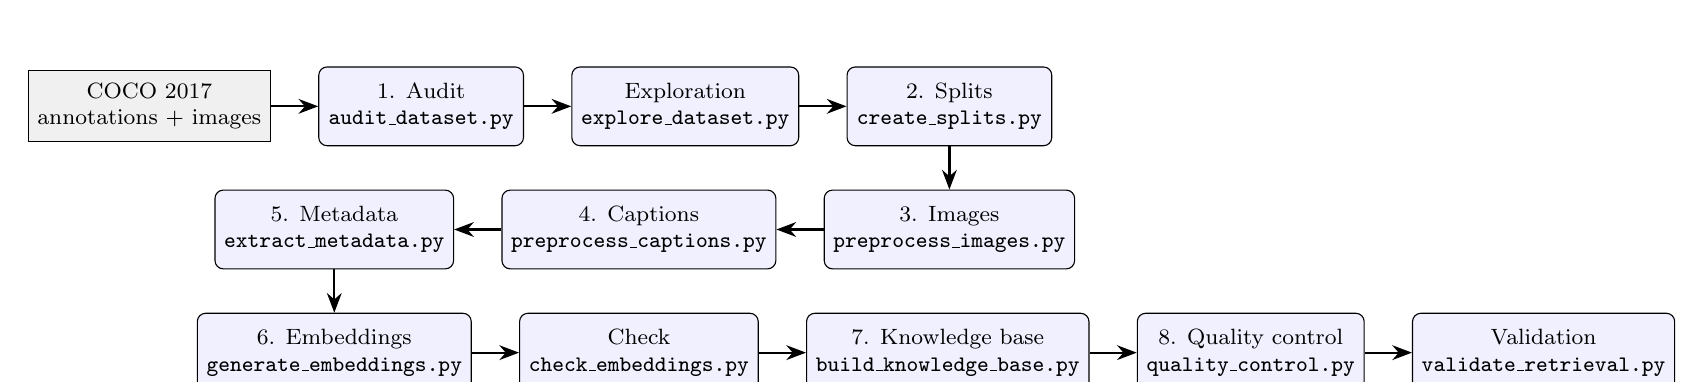
\begin{tikzpicture}[
  node distance=0.55cm and 0.6cm,
  box/.style={draw, rounded corners=3pt, fill=blue!6, minimum height=1.0cm, minimum width=2.6cm, align=center, font=\footnotesize},
  data/.style={draw, fill=gray!12, minimum height=0.9cm, minimum width=2.6cm, align=center, font=\footnotesize},
  arr/.style={-{Stealth[length=2.5mm]}, thick}
]
\node[data] (raw) {COCO 2017\\annotations + images};
\node[box, right=of raw] (audit) {1. Audit\\\code{audit\_dataset.py}};
\node[box, right=of audit] (explore) {Exploration\\\code{explore\_dataset.py}};
\node[box, right=of explore] (split) {2. Splits\\\code{create\_splits.py}};
\node[box, below=of split] (img) {3. Images\\\code{preprocess\_images.py}};
\node[box, left=of img] (cap) {4. Captions\\\code{preprocess\_captions.py}};
\node[box, left=of cap] (meta) {5. Metadata\\\code{extract\_metadata.py}};
\node[box, below=of meta] (emb) {6. Embeddings\\\code{generate\_embeddings.py}};
\node[box, right=of emb] (chk) {Check\\\code{check\_embeddings.py}};
\node[box, right=of chk] (kb) {7. Knowledge base\\\code{build\_knowledge\_base.py}};
\node[box, right=of kb] (qc) {8. Quality control\\\code{quality\_control.py}};
\node[box, right=of qc] (val) {Validation\\\code{validate\_retrieval.py}};
\draw[arr] (raw)--(audit); \draw[arr] (audit)--(explore); \draw[arr] (explore)--(split);
\draw[arr] (split)--(img); \draw[arr] (img)--(cap); \draw[arr] (cap)--(meta);
\draw[arr] (meta)--(emb); \draw[arr] (emb)--(chk); \draw[arr] (chk)--(kb); \draw[arr] (kb)--(qc); \draw[arr] (qc)--(val);
\end{tikzpicture}}
\caption{The Data Preparation and Knowledge Base Construction Pipeline
(Each box is an independent script; each arrow is a file dependency).}
\label{fig:pipeline}
\end{figure}



\subsection{Repository layout}

\begin{table}[H]
\centering
\small
\begin{tabular}{@{}>{\raggedright\arraybackslash}p{4.3cm}>{\raggedright\arraybackslash}p{10.5cm}@{}}
\toprule
\textbf{Directory} & \textbf{Content}\\
\midrule
\code{scripts/} & 25 Python scripts: the 11 pipeline scripts of Figure~\ref{fig:pipeline}, plus \code{explore\_knowledge\_base.py} (knowledge-base exploration), \code{create\_updated\_test\_split.py} and \code{check\_current\_splits.py} (test-set extension and split check), and the YOLO scripts (pilot, threshold experiment, full extraction, merge, checksums, tests).\\
\code{data/train2017/}, \code{data/val2017/} & Placeholders for the COCO 2017 images (not versioned; to be downloaded).\\
\code{data/annotations/} & Official COCO 2017 JSON files (captions, instances, person keypoints).\\
\code{data/splits/} & \code{knowledge\_base\_image\_ids.json}, \code{validation\_image\_ids.json}, \code{test\_image\_ids.json}.\\
\code{data/processed\_images/} & Pre-processed knowledge-base images (RGB, EXIF-corrected).\\
\code{data/captions/} & \code{kb\_captions\_raw.json} and \code{kb\_captions\_cleaned.json}.\\
\code{data/metadata/} & Objects, bounding boxes and spatial relations of the knowledge base (COCO ground truth).\\
\code{data/exploration/} & Outputs of the knowledge-base exploration (POS, colours, shapes, indoor/outdoor, day/night, COCO categories).\\
\code{data/visual\_detections/}, \code{data/visual\_detections\_test/} & YOLO detections: 100-image pilot, full 10\,000-image extraction, threshold and COCO-comparison experiments.\\
\code{data/embeddings/} & CLIP image and text embeddings (\code{.npy}) with ID mappings.\\
\code{data/index/} & FAISS indexes and the knowledge-base descriptor.\\
\code{reports/} & Audit, exploration, pre-processing, quality-control, retrieval-validation and YOLO-merge reports.\\
\bottomrule
\end{tabular}
\caption{Repository layout.}
\end{table}

\subsection{Reproducibility measures}
\begin{itemize}[nosep]
  \item \textbf{Public repository}: \url{https://github.com/Serine205/rag-coco-image-captioning}.
  \item \textbf{Fixed random seed} (\code{SEED = 42}) for all random selections.
  \item \textbf{Frozen splits} stored as versioned JSON files of image IDs.
  \item \textbf{Relative paths} computed from the script location (\code{Path(\_\_file\_\_)}), so the project runs on any machine.
  \item \textbf{Every script writes a report} (JSON/CSV) so that each decision is traceable.
  \item \textbf{Git LFS} (\code{data/** filter=lfs}; every file under \code{data/} must be fetched with \code{git lfs pull}) is used for the large artefacts (annotations, embeddings, indexes); the raw and processed images are excluded from version control by \code{.gitignore} to avoid unnecessarily increasing the repository size, as the original COCO images can be downloaded again from the official dataset.
\end{itemize}




%====================================================================
\section{Datasets and splitting strategy}

\subsection{Datasets}
Two official splits of COCO 2017 are used:
\begin{itemize}[nosep]
  \item \textbf{COCO train2017}: 118\,287 images and 591\,753 captions, from which the 10\,000-image knowledge base and the 100-image tuning set are sampled;
  \item \textbf{COCO val2017}: 5\,000 images and 25\,014 captions, from which the evaluation (test) images are sampled.
\end{itemize}


\begin{table}[H]
\centering
\small
\renewcommand{\arraystretch}{1.15}
\begin{tabularx}{\textwidth}{@{}>{\raggedright\arraybackslash}p{4.6cm} >{\raggedright\arraybackslash}p{3.4cm} r >{\raggedright\arraybackslash}X@{}}
\toprule
\textbf{Usage} & \textbf{Source} & \textbf{Images} & \textbf{Output file}\\
\midrule
RAG knowledge base & train2017 & 10\,000 & \code{knowledge\_base\_image\_ids.json}\\
Hyper-parameter tuning (validation) & train2017 (disjoint from KB) & 100 & \code{validation\_image\_ids.json}\\
Test / evaluation & val2017 & 1\,000 & \code{test\_1000\_image\_ids.json}\\
Legacy test (kept) & val2017 & 100 & \code{test\_image\_ids.json}, \code{test\_100\_image\_ids\_legacy.json}\\
\bottomrule
\end{tabularx}
\caption{Splits implemented by \code{create\_splits.py} (the 1\,000-image test file is produced by \code{create\_updated\_test\_split.py}).}
\label{tab:splits}
\end{table}

\begin{remark}[Size of the test set]\label{sec:testsize}
The project statement is not consistent on this point: Sections~4.1 and 4.2 specify \textbf{100} test images, whereas Sections~4.4.2 and 4.4.3 mention \textbf{1\,000}. The repository was first built with 100 test images and then extended: \code{create\_updated\_test\_split.py} keeps the 100 original images (saved unchanged as \code{test\_100\_image\_ids\_legacy.json}) and adds 900 images drawn at random (seed 42) from the remaining val2017 images, giving \code{test\_1000\_image\_ids.json}. The script asserts that the 1\,000 images belong to val2017, include the legacy 100, and that the knowledge-base and validation sets are disjoint. The file \code{test\_image\_ids.json} was deliberately left untouched (still 100 images). The 1\,000-image file is therefore the reference test set of this release, while the figures of the formal quality-control report (Table~\ref{tab:qc}) were produced with the 100-image file.
\end{remark}


%====================================================================
\section{Step 1 --- Data audit and validation}
\label{sec:audit}

\subsection{Objective of the dataset audit}

Before starting data pre-processing and implementing the Retrieval-Augmented Generation (RAG) approaches, it is important to verify the quality and consistency of the MS COCO dataset, to ensure that the images and their corresponding annotations are correctly organised and that no structural problem could affect the subsequent stages of the project.

Several checks were performed to verify the completeness and consistency of the raw data: image counts, number of reference captions per image, missing, corrupted and duplicated images, and image--caption integrity (Section~4.4.3, step 1).

The audit results generated by \code{scripts/audit\_dataset.py} were saved in a JSON report named \code{dataset\_audit.json}, located in the \code{reports/} directory. This report contains the audit results for both datasets.


\subsection{Method (\code{audit\_dataset.py})}
For each of the two datasets, the script:
\begin{enumerate}[nosep]
  \item loads the COCO caption JSON and counts the physical \code{.jpg} files in the image directory;
  \item checks the uniqueness of image IDs (\code{duplicate\_ids});
  \item counts the captions per image (\code{Counter} over \code{image\_id}) and builds the distribution of this count; images whose count differs from 5 are flagged;
  \item for each image listed in the annotations, builds the file name \code{\{id:012d\}.jpg}; a missing file is recorded as \emph{missing}; otherwise the file is opened with PIL and \code{Image.verify()} is called -- an exception marks the image as \emph{corrupted};
  \item computes the \textbf{SHA-256 hash of each file}; identical hashes reveal \textbf{exact duplicate images};
  \item detects \emph{orphan captions}, i.e. captions whose \code{image\_id} is absent from the image list.
\end{enumerate}

\subsection{Results}
\begin{table}[H]
\centering
\begin{tabular}{@{}lrr@{}}
\toprule
\textbf{Indicator} & \textbf{train2017} & \textbf{val2017}\\
\midrule
Physical images & 118\,287 & 5\,000\\
Images in annotations & 118\,287 & 5\,000\\
Total captions & 591\,753 & 25\,014\\
Duplicate image IDs & 0 & 0\\
Images with exactly 5 captions & 117\,972 & 4\,987\\
Images with 6 captions & 312 & 12\\
Images with 7 captions & 3 & 1\\
Images with $\neq 5$ captions & 315 & 13\\
Missing images & 0 & 0\\
Corrupted images & 0 & 0\\
Groups of exact duplicate images (SHA-256) & 12 & 0\\
Orphan captions & 0 & 0\\
\bottomrule
\end{tabular}
\caption{Dataset audit (source: \code{reports/dataset\_audit.json}).}
\label{tab:audit}
\end{table}

\subsection{Interpretation}
\begin{interp}
\begin{itemize}[nosep]
  \item \textbf{Completeness.} Both datasets are complete: the number of physical images equals the number of images declared in the annotations, with no missing, corrupted or orphan item. No sample had to be removed, so the rule ``remove invalid samples only if documented'' is trivially satisfied.
  \item \textbf{Captions per image.} The ``5 captions per image'' rule holds for 99.73\,\% of train2017 (117\,972/118\,287) and 99.74\,\% of val2017 (4\,987/5\,000). The few exceptions have \emph{more} captions (6 or 7), never fewer: $591\,753-5\times118\,287=318$ extra captions $=312\times1+3\times2$, which matches the table exactly. No image lacks references.
  \item \textbf{Consequence for the project.} Because some images carry 6 or 7 captions, the statement's ``50\,000 captions in the knowledge base'' becomes 50\,028 in practice (Section~\ref{sec:captions}). We deliberately keep \emph{all} reference captions rather than truncating to 5: truncating would silently discard human annotations and would require an arbitrary choice.
  \item \textbf{Duplicates.} 12 groups of byte-identical images exist in train2017 (none in val2017). Their effect is negligible at the scale of 118\,287 images, but a duplicate present both in the knowledge base and in the tuning set would be a subtle form of leakage; this point is listed among the limitations (Section~\ref{sec:limits}).
\end{itemize}
\end{interp}


%====================================================================
\section{Statistical exploration of the dataset}
\label{sec:explore}

\subsection{Objective and scope}
The statistical exploration aims to provide a documented analysis covering: (i) object-class distribution (top 50), (ii) scene complexity, (iii) textual statistics, (iv) diversity analysis, (v) visualisations. The analysis is implemented in \code{explore\_dataset.py} and is applied to the \textbf{complete COCO train2017 set} (118\,287 images), which is the population from which the knowledge base is drawn. Working on the full population gives stable statistics and shows what a random 10\,000-image sample is expected to look like.
All generated results, including CSV files, the JSON summary, and visualisations, are saved in the \code{reports/exploration/} directory.

\subsection{Method}
\begin{itemize}[nosep]
  \item \textbf{Captions} (\code{captions\_train2017.json}): the caption length is the number of tokens found by the regular expression \verb|\b\w+\b|; for the vocabulary and the total word count, captions are lower-cased and words are extracted with \verb|[a-zA-Z]+| (a different tokenisation from the one used for the caption length, hence slightly different totals). We then compute the total word count, the vocabulary size, the mean / median / min / max length and the word frequencies (\code{collections.Counter}).
  \item \textbf{Objects} (\code{instances\_train2017.json}): each annotation carries a \code{category\_id} that is mapped to its name; we count annotations per category, annotations per image, and the set of categories present in each image.
  \item \textbf{Co-occurrence}: for each image, every unordered pair of distinct categories is counted once (\code{itertools.combinations}); the 20 most frequent pairs are exported.
  \item \raggedright\textbf{Outputs}: CSV tables (\code{top\_50\_objects.csv}, \code{top\_words.csv}, \code{object\_cooccurrence.csv}), a JSON summary (\code{exploration\_summary.json}) and four 300-dpi figures.
\end{itemize}

\subsection{Distribution of object classes}

COCO annotates \textbf{80 object categories}; train2017 contains \textbf{860\,001 object annotations}. Table~\ref{tab:top50} gives the top 50 categories and Figure~\ref{fig:top20} shows the top 20.

\begin{figure}[H]
\centering
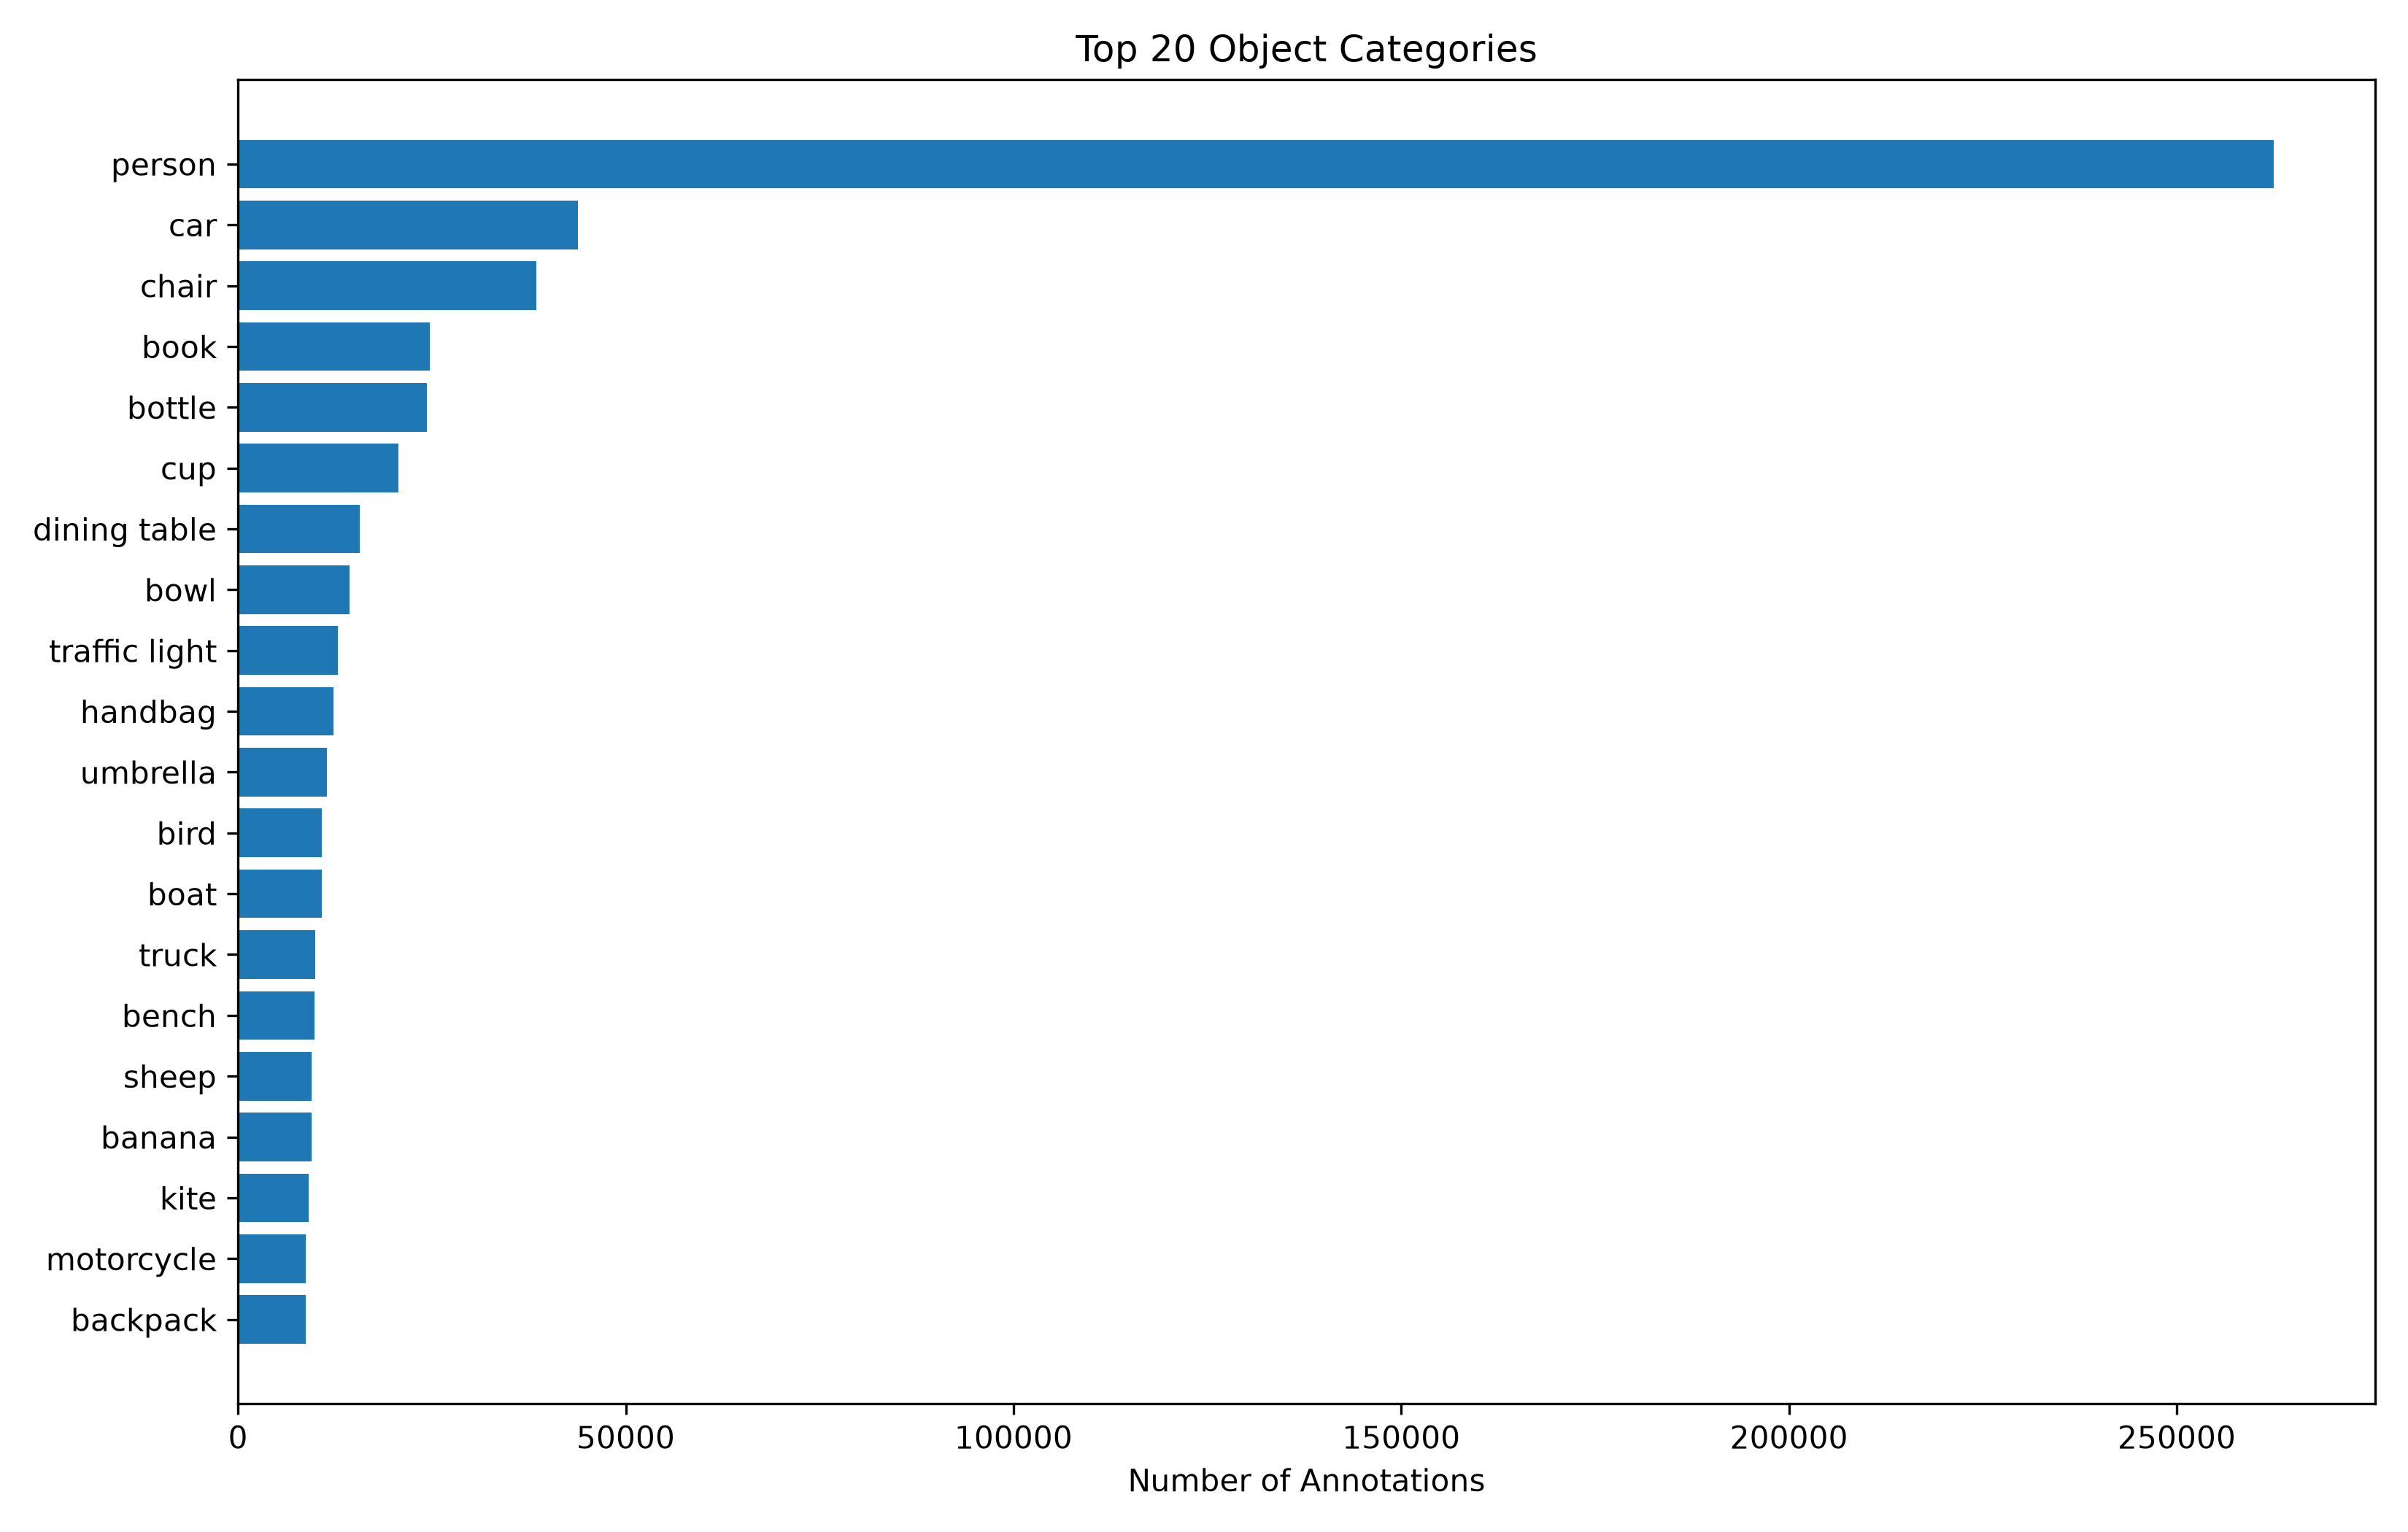
\includegraphics[width=0.88\textwidth]{figures/top_20_objects.png}
\caption{Top 20 object categories in COCO train2017 (number of annotations).}
\label{fig:top20}
\end{figure}

{\small
\begin{longtable}{@{}rlr rlr rlr@{}}
\caption{Top 50 object categories (number of annotations, train2017).}\label{tab:top50}\\
\toprule
\# & \textbf{Category} & \textbf{Freq.} & \# & \textbf{Category} & \textbf{Freq.} & \# & \textbf{Category} & \textbf{Freq.}\\
\midrule
\endfirsthead
\toprule
\# & \textbf{Category} & \textbf{Freq.} & \# & \textbf{Category} & \textbf{Freq.} & \# & \textbf{Category} & \textbf{Freq.}\\
\midrule
\endhead
1 & person & 262\,465 & 18 & kite & 9\,076 & 35 & cake & 6\,353\\
2 & car & 43\,867 & 19 & motorcycle & 8\,725 & 36 & sports ball & 6\,347\\
3 & chair & 38\,491 & 20 & backpack & 8\,720 & 37 & clock & 6\,334\\
4 & book & 24\,715 & 21 & potted plant & 8\,652 & 38 & suitcase & 6\,192\\
5 & bottle & 24\,342 & 22 & cow & 8\,147 & 39 & spoon & 6\,165\\
6 & cup & 20\,650 & 23 & wine glass & 7\,913 & 40 & surfboard & 6\,126\\
7 & dining table & 15\,714 & 24 & carrot & 7\,852 & 41 & bus & 6\,069\\
8 & bowl & 14\,358 & 25 & knife & 7\,770 & 42 & apple & 5\,851\\
9 & traffic light & 12\,884 & 26 & broccoli & 7\,308 & 43 & pizza & 5\,821\\
10 & handbag & 12\,354 & 27 & donut & 7\,179 & 44 & tv & 5\,805\\
11 & umbrella & 11\,431 & 28 & bicycle & 7\,113 & 45 & couch & 5\,779\\
12 & bird & 10\,806 & 29 & skis & 6\,646 & 46 & remote & 5\,703\\
13 & boat & 10\,759 & 30 & vase & 6\,613 & 47 & sink & 5\,610\\
14 & truck & 9\,973 & 31 & horse & 6\,587 & 48 & skateboard & 5\,543\\
15 & bench & 9\,838 & 32 & tie & 6\,496 & 49 & elephant & 5\,513\\
16 & sheep & 9\,509 & 33 & cell phone & 6\,434 & 50 & dog & 5\,508\\
17 & banana & 9\,458 & 34 & orange & 6\,399 & & & \\
\bottomrule
\end{longtable}}

\begin{interp}
\begin{itemize}[nosep]
  \item \textbf{Very strong class imbalance (long tail).} The class \emph{person} alone accounts for $262\,465/860\,001=\mathbf{30.5\,\%}$ of all annotations, i.e. 2.2 persons per image on average and about 6 times more than the second class (car, 43\,867). The top 3, top 5 and top 10 classes cover 40.1\,\%, 45.8\,\% and 54.6\,\% of annotations; the top 50 cover 88.8\,\%, so the 30 remaining classes share only 11.2\,\%.
  \item \textbf{Everyday-life dominance.} The most frequent classes are urban and domestic objects (car, chair, book, bottle, cup, dining table, traffic light, handbag). Typical COCO scenes are therefore streets, kitchens, dining rooms and sports fields.
  \item \textbf{Implication for captioning and RAG.} A captioner and a retriever will see ``person'' evidence in a majority of images; the retrieved neighbours will tend to share this class, which can make retrieval look good for trivial reasons. For hallucination analysis (Section~10.4 of the statement), \emph{rare} classes (the tail of the distribution) are where a model is most likely to omit or invent objects, so error rates should be reported per frequency band, not only globally.
  \item \textbf{Metadata filtering (G28--G30).} For metadata-filtered RAG, a filter on ``person'' is almost non-selective, whereas a filter on a tail class (e.g. elephant, 5\,513 annotations) is very selective; the choice of filtering strategy (strict vs. boosting) will thus depend strongly on the class frequency.
\end{itemize}
\end{interp}

\subsection{Scene complexity}

\paragraph{Objects per image.} The mean number of object annotations per image is $860\,001/118\,287=\mathbf{7.27}$. Figure~\ref{fig:objperimg} shows the distribution.

\begin{figure}[H]
\centering
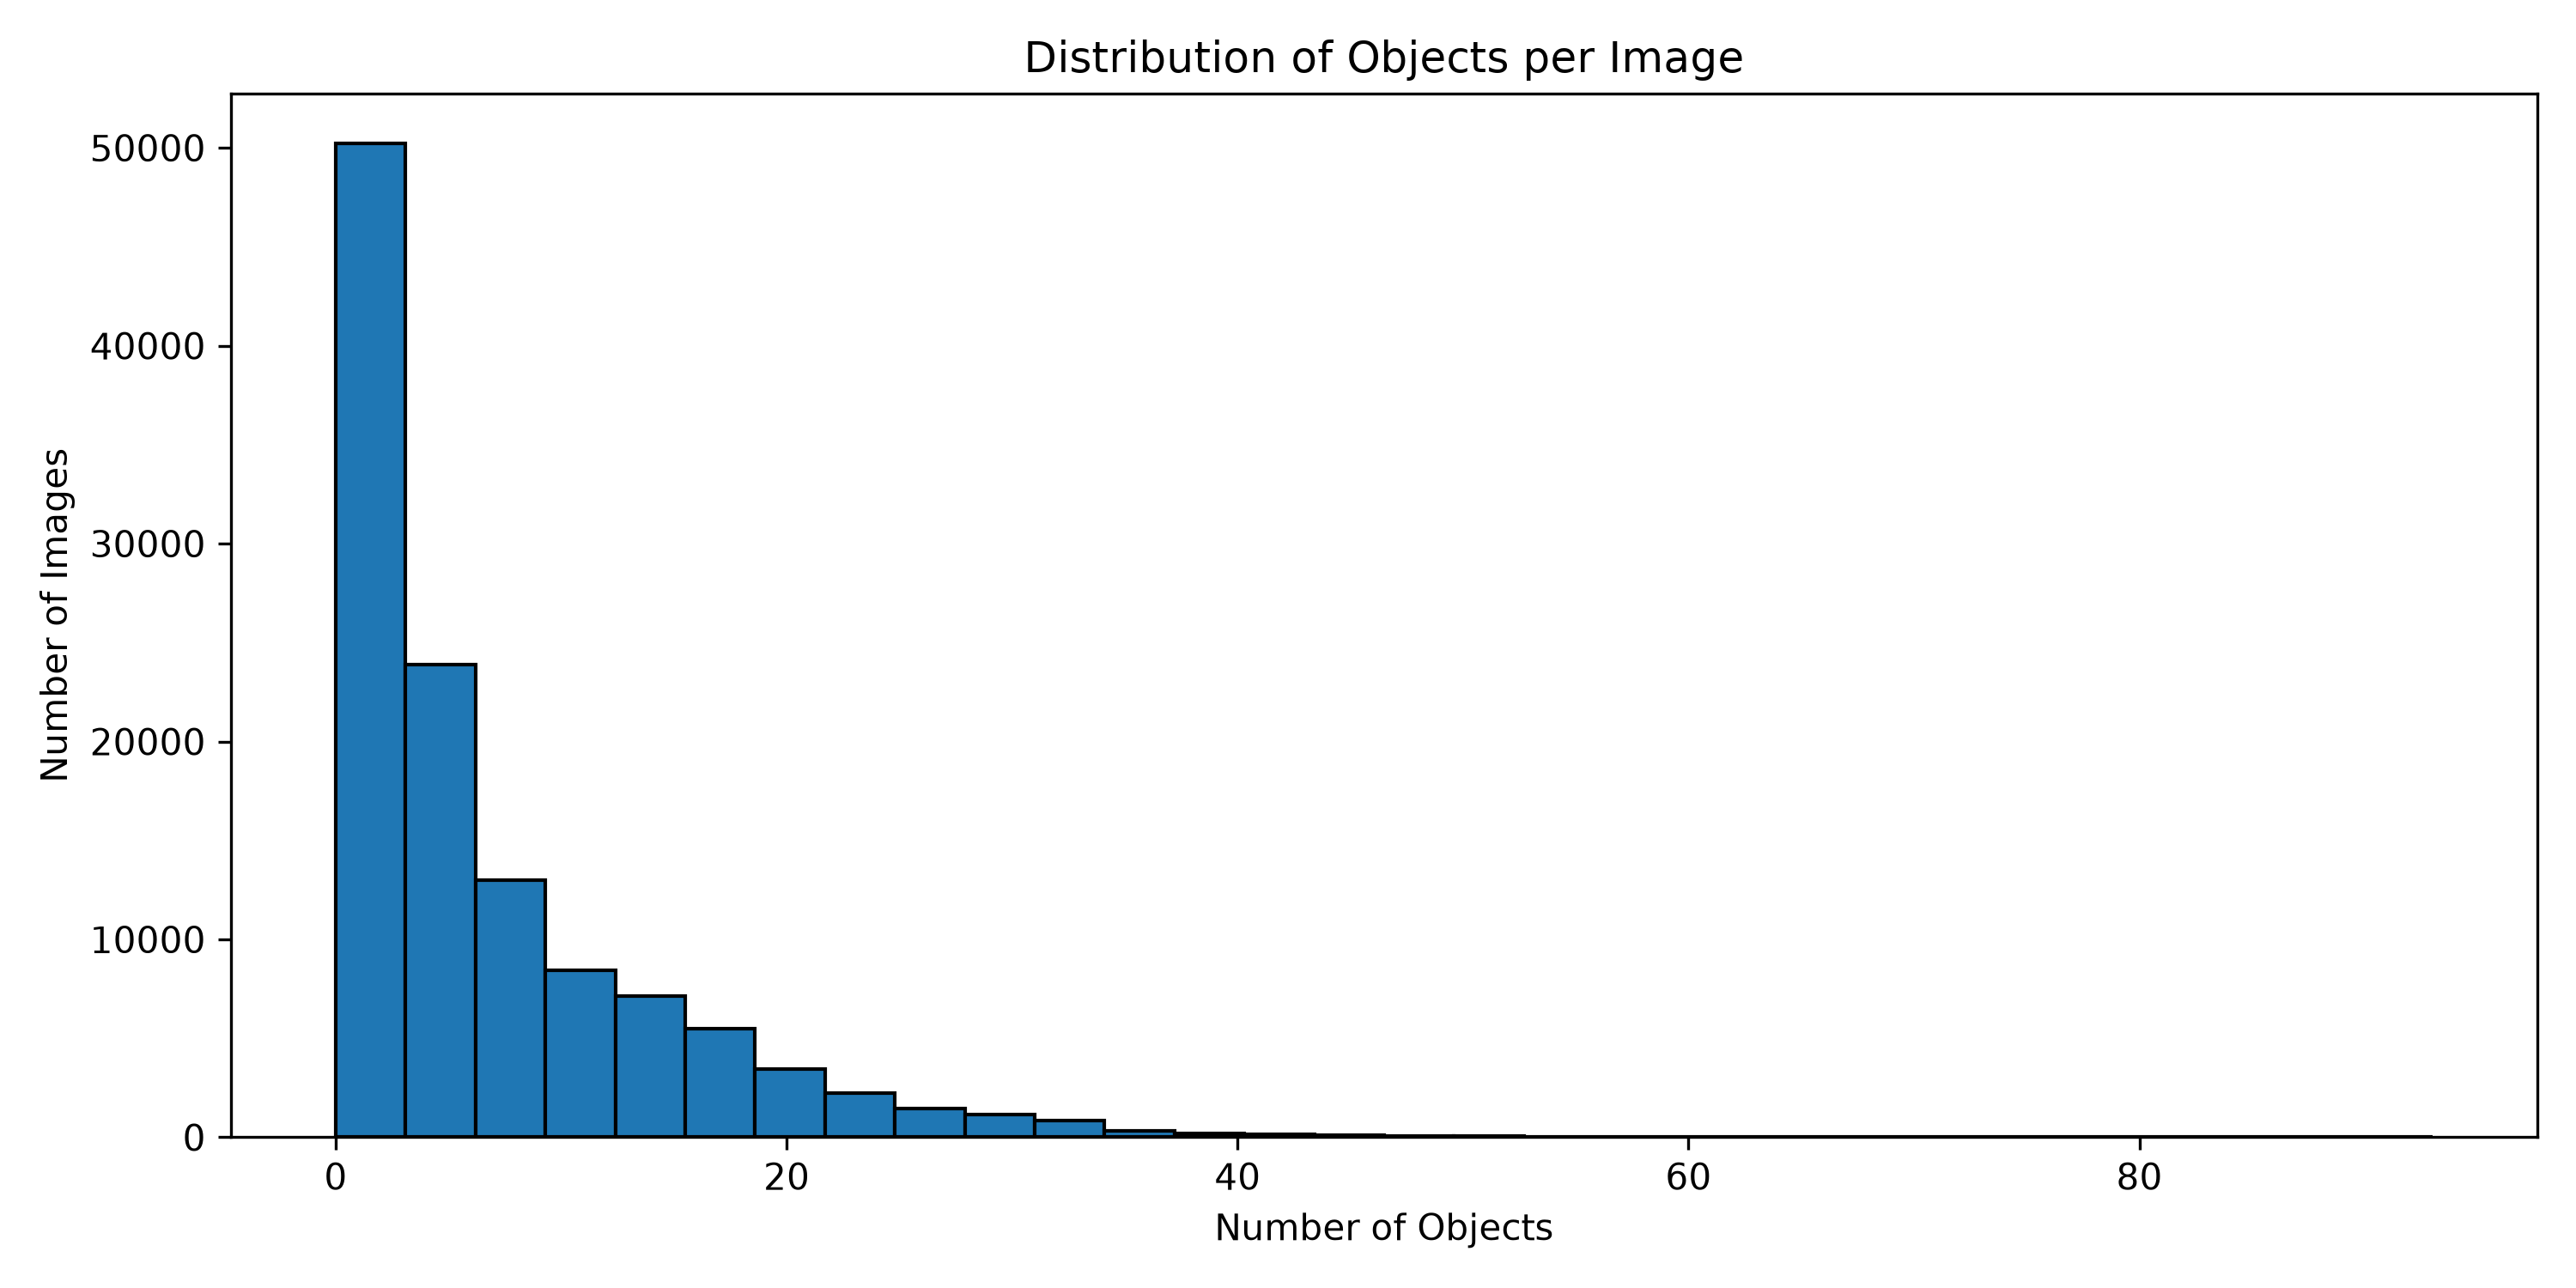
\includegraphics[width=0.85\textwidth]{figures/objects_per_image.png}
\caption{Distribution of the number of annotated objects per image (train2017).}
\label{fig:objperimg}
\end{figure}

\begin{interp}
The distribution is strongly \textbf{right-skewed} (long tail up to about 90 objects): the first bin (0--3 objects) contains roughly 50\,000 images, i.e. about 42\,\% of the dataset, and the frequency decreases quickly afterwards (about 24\,000 images in the 3--6 bin, 13\,000 in the 6--9 bin). The mean (7.27) is therefore larger than the typical (modal) scene, which contains only a few objects. COCO thus mixes \emph{simple scenes} (a few salient objects) and \emph{complex scenes} (crowds, kitchens, streets with tens of instances). This confirms that the test subset must be \textbf{stratified} on scene complexity, as required by the statement, otherwise a random 100-image sample could be dominated by simple scenes and hide failures on cluttered ones. Complex scenes are also where \emph{object hallucination} and \emph{omission} are most likely.
\end{interp}

\paragraph{Object co-occurrence and spatial relations.} Table~\ref{tab:cooc} reports the 20 most frequent unordered pairs of categories appearing together in the same image.

\begin{table}[H]
\centering
\small
\begin{tabular}{@{}rllr@{\hspace{1.2cm}}rllr@{}}
\toprule
\# & \textbf{Object 1} & \textbf{Object 2} & \textbf{Images} & \# & \textbf{Object 1} & \textbf{Object 2} & \textbf{Images}\\
\midrule
1 & car & person & 8\,519 & 11 & person & sports ball & 4\,097\\
2 & chair & person & 8\,035 & 12 & person & truck & 3\,992\\
3 & handbag & person & 6\,222 & 13 & cell phone & person & 3\,830\\
4 & dining table & person & 5\,869 & 14 & car & truck & 3\,664\\
5 & chair & dining table & 5\,124 & 15 & person & tie & 3\,632\\
6 & backpack & person & 5\,034 & 16 & person & umbrella & 3\,447\\
7 & cup & person & 4\,848 & 17 & person & skateboard & 3\,417\\
8 & cup & dining table & 4\,679 & 18 & bowl & dining table & 3\,396\\
9 & bottle & person & 4\,561 & 19 & person & surfboard & 3\,365\\
10 & bench & person & 4\,108 & 20 & person & tennis racket & 3\,361\\
\bottomrule
\end{tabular}
\caption{Top 20 object co-occurrences (number of images containing both categories).}
\label{tab:cooc}
\end{table}

\begin{interp}
Co-occurrences reflect \textbf{real-world contexts}: person+car / person+handbag (street), chair+dining table+cup+bowl (indoor dining), person+sports ball / skateboard / surfboard / tennis racket (sports), car+truck (road traffic). 16 of the 20 pairs include ``person'', which is expected given its frequency. These strong contextual priors are a double-edged sword for captioning: they let a model infer plausible objects (useful for RAG), but also cause \emph{hallucination by association} (e.g. mentioning a ``chair'' because a ``dining table'' is visible). They also justify the \textbf{spatial relations} extracted in Step~5 (Section~\ref{sec:metadata}): left/right and above/below relations are computed between the bounding boxes of co-occurring objects.
\end{interp}


\subsection{Textual statistics}

\begin{table}[H]
\centering
\begin{tabular}{@{}lr@{}}
\toprule
\textbf{Statistic} & \textbf{Value}\\
\midrule
Total captions & 591\,753\\
Total words & 6\,199\,120\\
Vocabulary size (distinct lower-cased words) & 26\,466\\
Mean caption length (words) & 10.48\\
Median caption length (words) & 10.0\\
Minimum / maximum caption length & 5 / 50\\
Type/token ratio ($26\,466/6\,199\,120$) & 0.43\,\%\\
Captions per image (mean) & 5.003\\
\bottomrule
\end{tabular}
\caption{Caption statistics on train2017 (source: \code{exploration\_summary.json}).}
\label{tab:textstats}
\end{table}

\begin{figure}[H]
\centering
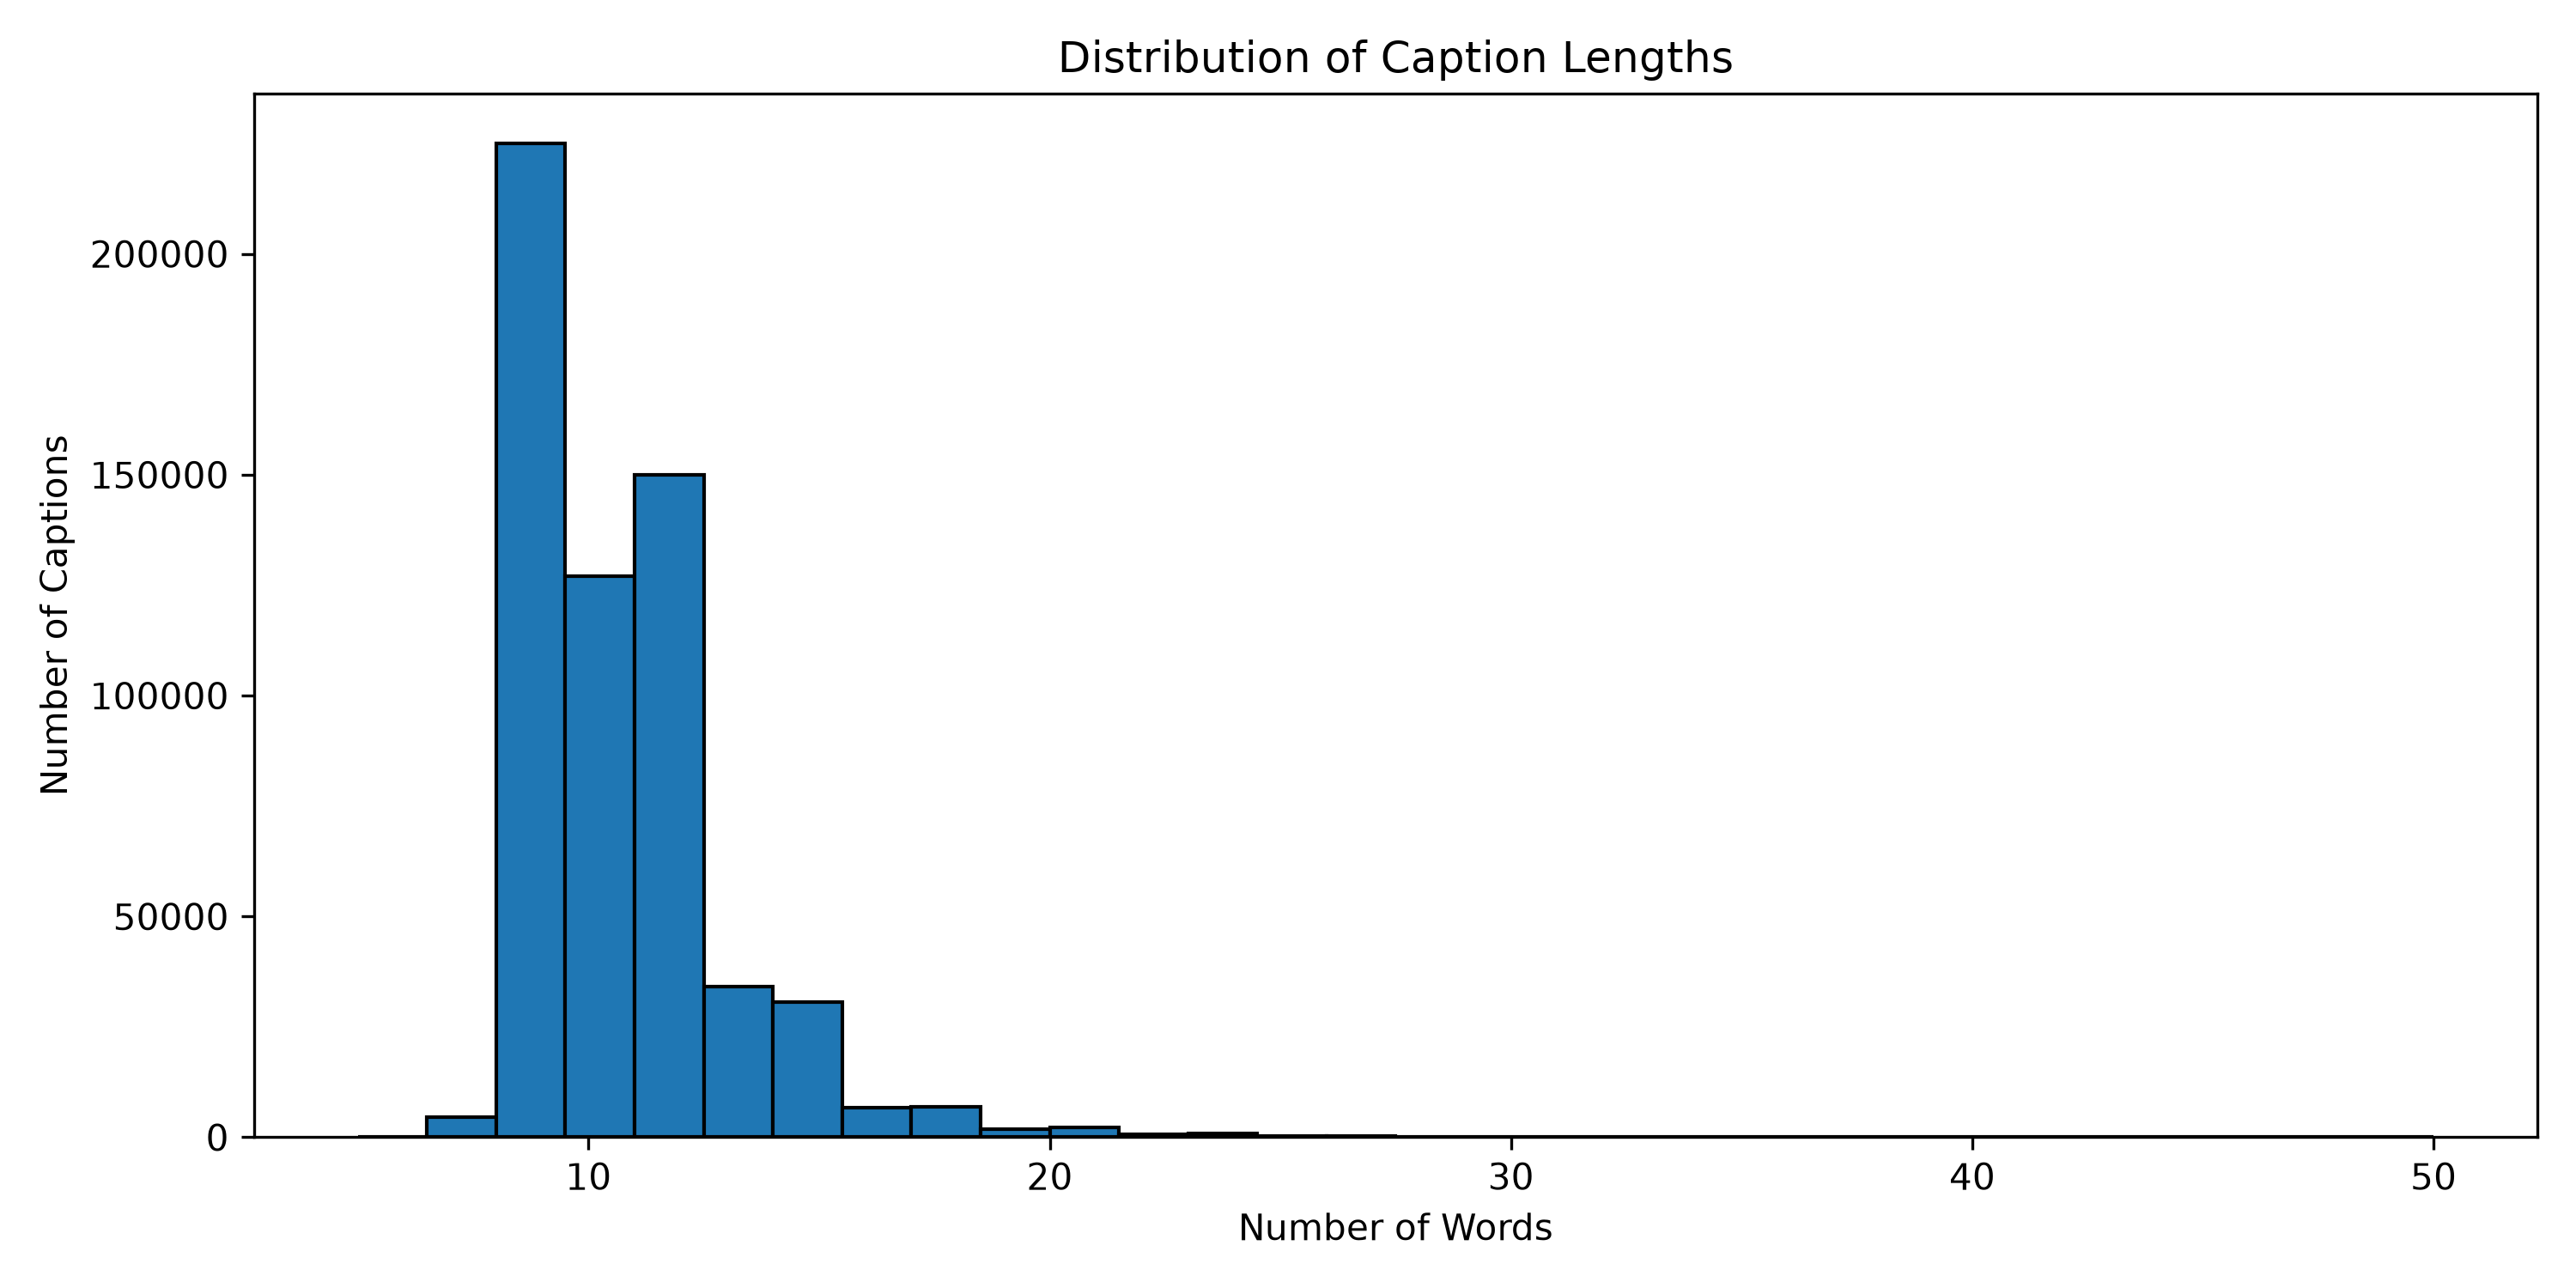
\includegraphics[width=0.85\textwidth]{figures/caption_lengths.png}
\caption{Distribution of caption lengths (words).}
\label{fig:caplen}
\end{figure}

\begin{interp}
\begin{itemize}[nosep]
  \item \textbf{Short, homogeneous captions.} Mean 10.48 and median 10 words, with the bulk between 8 and 13 words (histogram modes at 9--10 and 12). The minimum is 5 and the long tail ends at 50 words, but captions above 20 words are very rare. This is consistent with COCO's annotation protocol (one sentence describing the main scene).
  \item \textbf{Compatibility with the encoder.} CLIP's text encoder accepts at most 77 tokens. Since almost all captions are under 20 words, truncation (\code{max\_length=77}, \code{truncation=True}) can only affect a handful of extreme outliers (the longest caption has 50 words, which may approach the 77-token limit once punctuation and sub-word splitting are counted).
  \item \textbf{Reference length for generation.} A generated caption is expected to be about 10 words long. Models that produce much longer captions will be penalised by BLEU/CIDEr (length mismatch), so the generation length should be controlled during hyper-parameter tuning.
  \item \textbf{Low lexical diversity ratio.} The vocabulary (26\,466 words) is small relative to the 6.2\,M tokens (type/token ratio 0.43\,\%): captions reuse a restricted, repetitive vocabulary. This favours lexical retrieval such as BM25 on the knowledge-base captions, because query words are likely to occur in the corpus.
\end{itemize}
\end{interp}

\paragraph{Most frequent words.} Figure~\ref{fig:topwords} and Table~\ref{tab:topwords} give the most frequent words.

\begin{figure}[H]
\centering
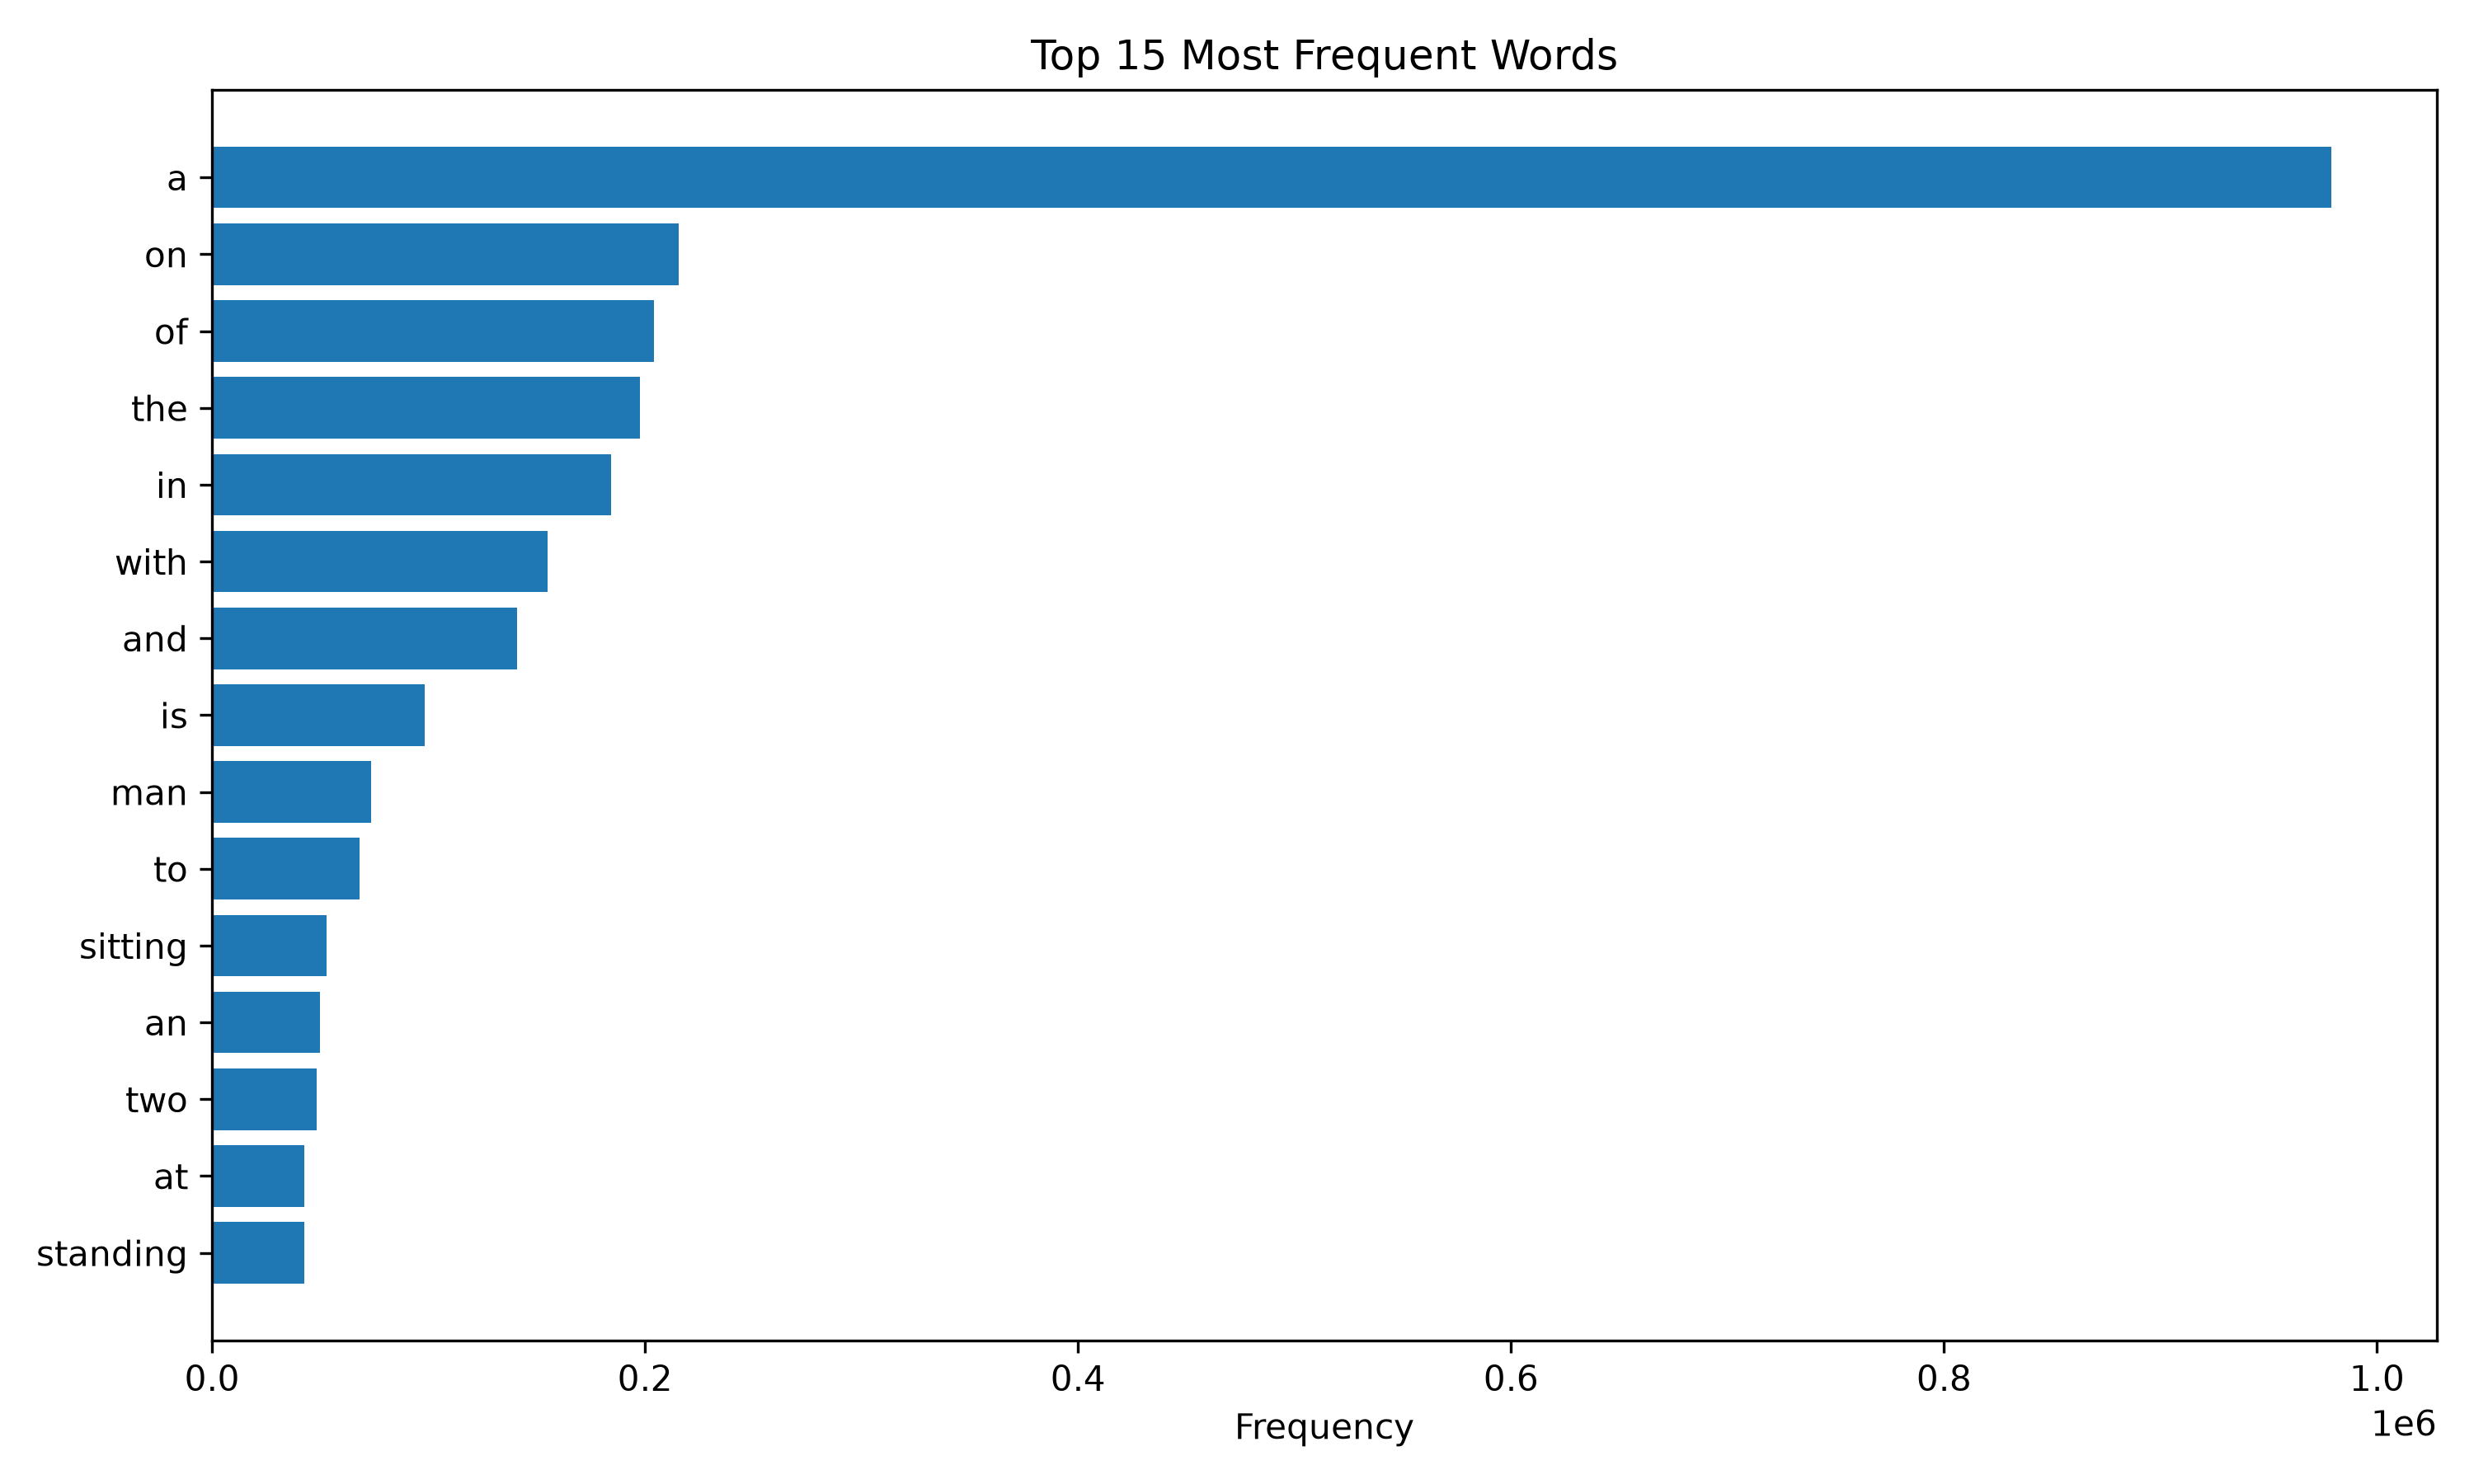
\includegraphics[width=0.82\textwidth]{figures/top_words.png}
\caption{Top 15 most frequent words in captions (frequency $\times 10^6$).}
\label{fig:topwords}
\end{figure}

\begin{table}[H]
\centering
\small
\begin{tabular}{@{}rlr@{\hspace{0.8cm}}rlr@{\hspace{0.8cm}}rlr@{}}
\toprule
\# & \textbf{Word} & \textbf{Freq.} & \# & \textbf{Word} & \textbf{Freq.} & \# & \textbf{Word} & \textbf{Freq.}\\
\midrule
1 & a & 978\,685 & 11 & sitting & 52\,911 & 21 & street & 30\,291\\
2 & on & 215\,689 & 12 & an & 49\,875 & 22 & table & 30\,187\\
3 & of & 204\,072 & 13 & two & 48\,404 & 23 & that & 28\,175\\
4 & the & 197\,771 & 14 & at & 42\,724 & 24 & holding & 27\,968\\
5 & in & 184\,143 & 15 & standing & 42\,485 & 25 & it & 26\,981\\
6 & with & 154\,811 & 16 & people & 41\,939 & 26 & person & 24\,745\\
7 & and & 140\,916 & 17 & are & 41\,086 & 27 & large & 24\,556\\
8 & is & 98\,184 & 18 & next & 37\,215 & 28 & some & 24\,330\\
9 & man & 73\,340 & 19 & white & 36\,364 & 29 & down & 23\,140\\
10 & to & 68\,161 & 20 & woman & 34\,210 & 30 & top & 22\,299\\
\bottomrule
\end{tabular}
\caption{Top 30 words in the reference captions (train2017).}
\label{tab:topwords}
\end{table}

\begin{interp}
\begin{itemize}[nosep]
  \item \textbf{Function words dominate.} The article ``a'' alone represents 15.8\,\% of all tokens; the top 10 words represent 37.4\,\% and the top 30 represent 48.5\,\%. In the list, 12 of the first 20 words are function words (articles, prepositions, conjunctions, auxiliaries). This has direct consequences for \textbf{BM25 and sparse retrieval}: stop-words carry almost no discriminative information and must be handled by IDF weighting or removed in the sparse index.
  \item \textbf{Content words reveal the dataset's semantics.} Among content words, \emph{man}, \emph{woman}, \emph{people}, \emph{person} (persons), \emph{sitting}, \emph{standing}, \emph{holding} (actions/postures), \emph{two} (counting), \emph{white} (colour), \emph{street}, \emph{table}, \emph{top} (places and spatial terms) dominate. Captions therefore describe mostly \textbf{people, their posture, their location and a few attributes}, which agrees with the object statistics (``person'' $=30.5\,\%$ of annotations).
  \item \textbf{Spatial and relational vocabulary.} The words \emph{on}, \emph{in}, \emph{at}, \emph{next} (to), \emph{down}, \emph{top} (of) show that captions encode spatial relations frequently: relational hallucinations (wrong preposition / position) are a real risk to evaluate.
\end{itemize}
\end{interp}

\subsection{Diversity analysis}

The statement asks for an analysis of attributes (colour, shapes) and contexts (indoor/outdoor, day/night). No pixel-level attribute classifier is used: colours and shapes are extracted from the captions and the indoor/outdoor and day/night contexts are predicted with CLIP (Section~\ref{sec:explore-kb}). Combined with the object statistics, the diversity is characterised as follows:
\begin{itemize}[nosep]
  \item \textbf{Object diversity}: 80 categories, with a strong long tail (see above), plus 7.27 objects per image on average.
  \item \textbf{Context diversity}: besides the CLIP predictions of Section~\ref{sec:explore-kb}, indoor contexts are indicated by categories and words such as \emph{chair}, \emph{dining table}, \emph{couch}, \emph{sink}, \emph{tv}, \emph{book}, \emph{cup}, \emph{bowl}; outdoor contexts by \emph{car}, \emph{traffic light}, \emph{bench}, \emph{boat}, \emph{kite}, \emph{surfboard}, \emph{skis}, \emph{elephant}, \emph{street}. Both families are well represented in the top 50, which indicates a balanced mixture of indoor and outdoor scenes rather than one dominant setting.
  \item \textbf{Attribute diversity}: the only colour word in the top-30 words is \emph{white} (36\,364 occurrences, rank 19), and the size adjective \emph{large} (rank 27). The other colours appear beyond the 30 exported words; COCO captions therefore contain attributes, but in a minor proportion relative to objects and actions.
  \item \textbf{Visual diversity of the knowledge base}: Section~\ref{sec:images} reports the distribution of image resolutions and aspect ratios of the 10\,000 KB images.
\end{itemize}


\subsection{Exploration of the knowledge base}
\label{sec:explore-kb}
The statistics above describe the whole of train2017. A second script, \code{explore\_knowledge\_base.py}, analyses the 10\,000 knowledge-base images and their 50\,028 cleaned captions and covers what the first script does not: part-of-speech (POS) distribution, colours, shapes, and indoor/outdoor and day/night contexts. Outputs are stored in \code{data/exploration/} (CSV and JSON) and the figures in \code{reports/exploration/}.
\begin{itemize}[nosep]
  \item \textbf{POS distribution}: spaCy (\code{en\_core\_web\_sm}) tags every caption token (spaces and punctuation excluded); nouns, verbs and adjectives are counted by lemma (top 20 each).
  \item \textbf{Colours and shapes}: lexical extraction from the captions with fixed vocabularies (11 colours, 8 shapes, with synonyms such as \emph{grey}/\emph{gray}). These are the colours \emph{mentioned} by annotators, not measured on pixels.
  \item \textbf{Indoor/outdoor and day/night}: zero-shot classification of each image with CLIP ViT-B/32 (cosine similarity between the stored image embedding and two text prompts; the higher score gives the label). These labels are predictions, not verified ground truth.
  \item \textbf{COCO categories}: categories, super-categories, objects per image and category co-occurrences computed on the knowledge base (files \code{coco\_*.csv}).
\end{itemize}

\begin{figure}[H]
\centering
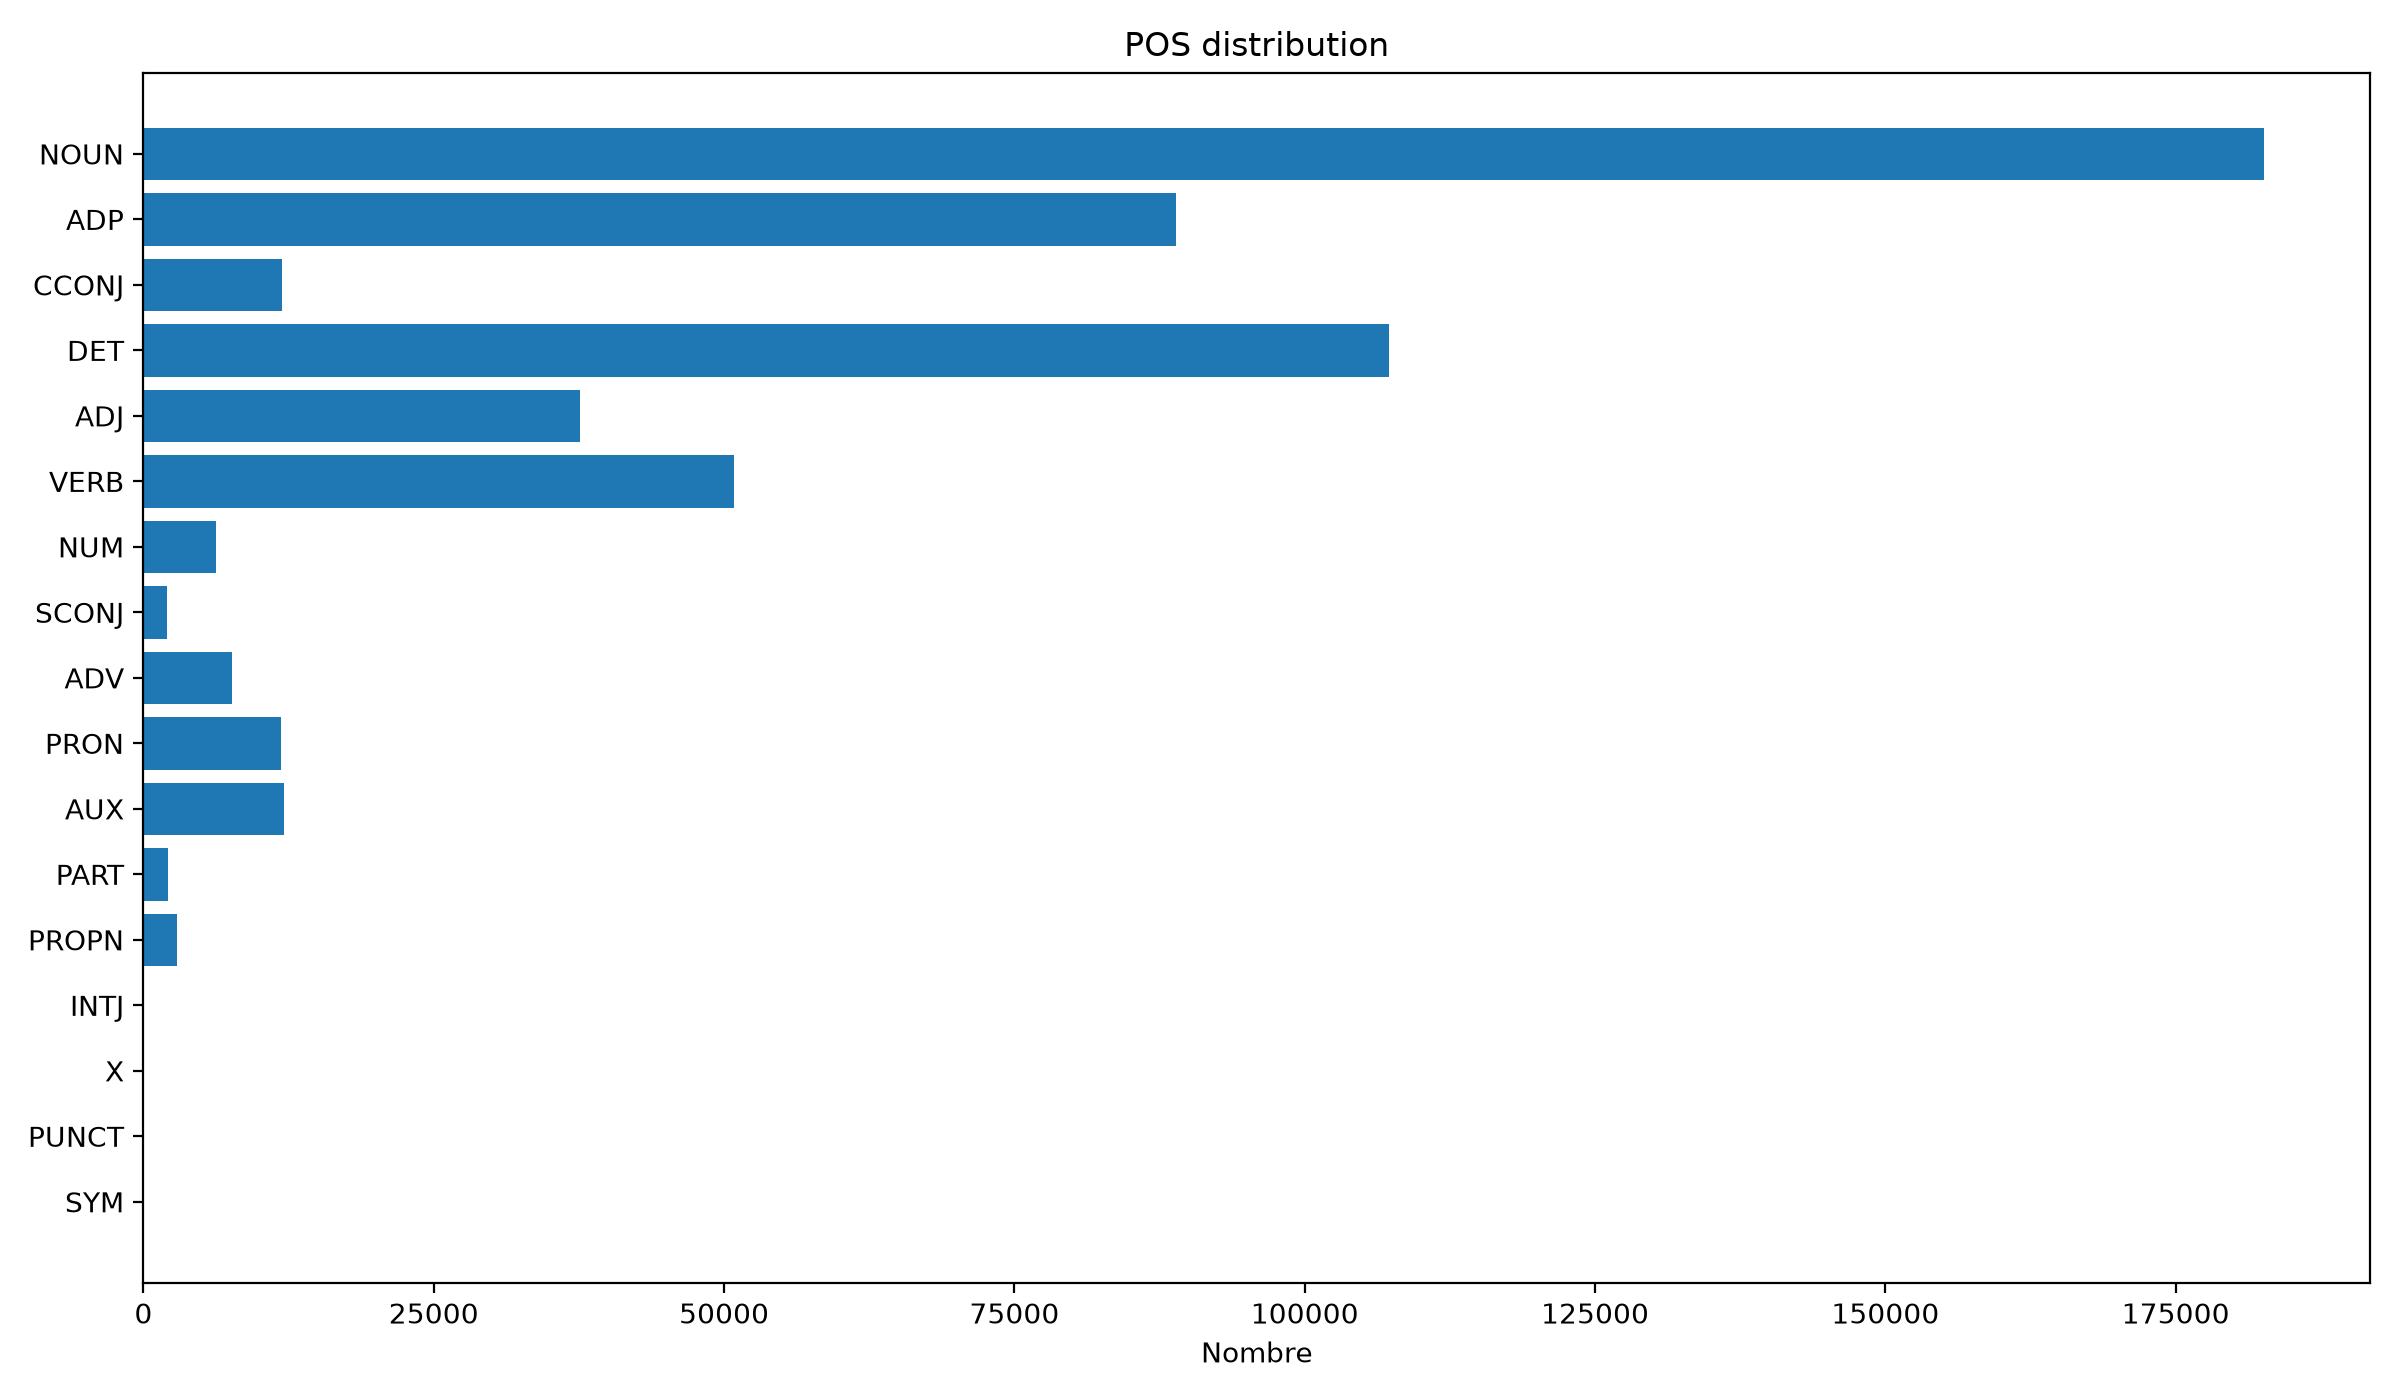
\includegraphics[width=0.78\textwidth]{figures/pos_distribution.png}
\caption{POS distribution of the knowledge-base captions (spaCy).}
\label{fig:pos}
\end{figure}

\begin{figure}[H]
\centering
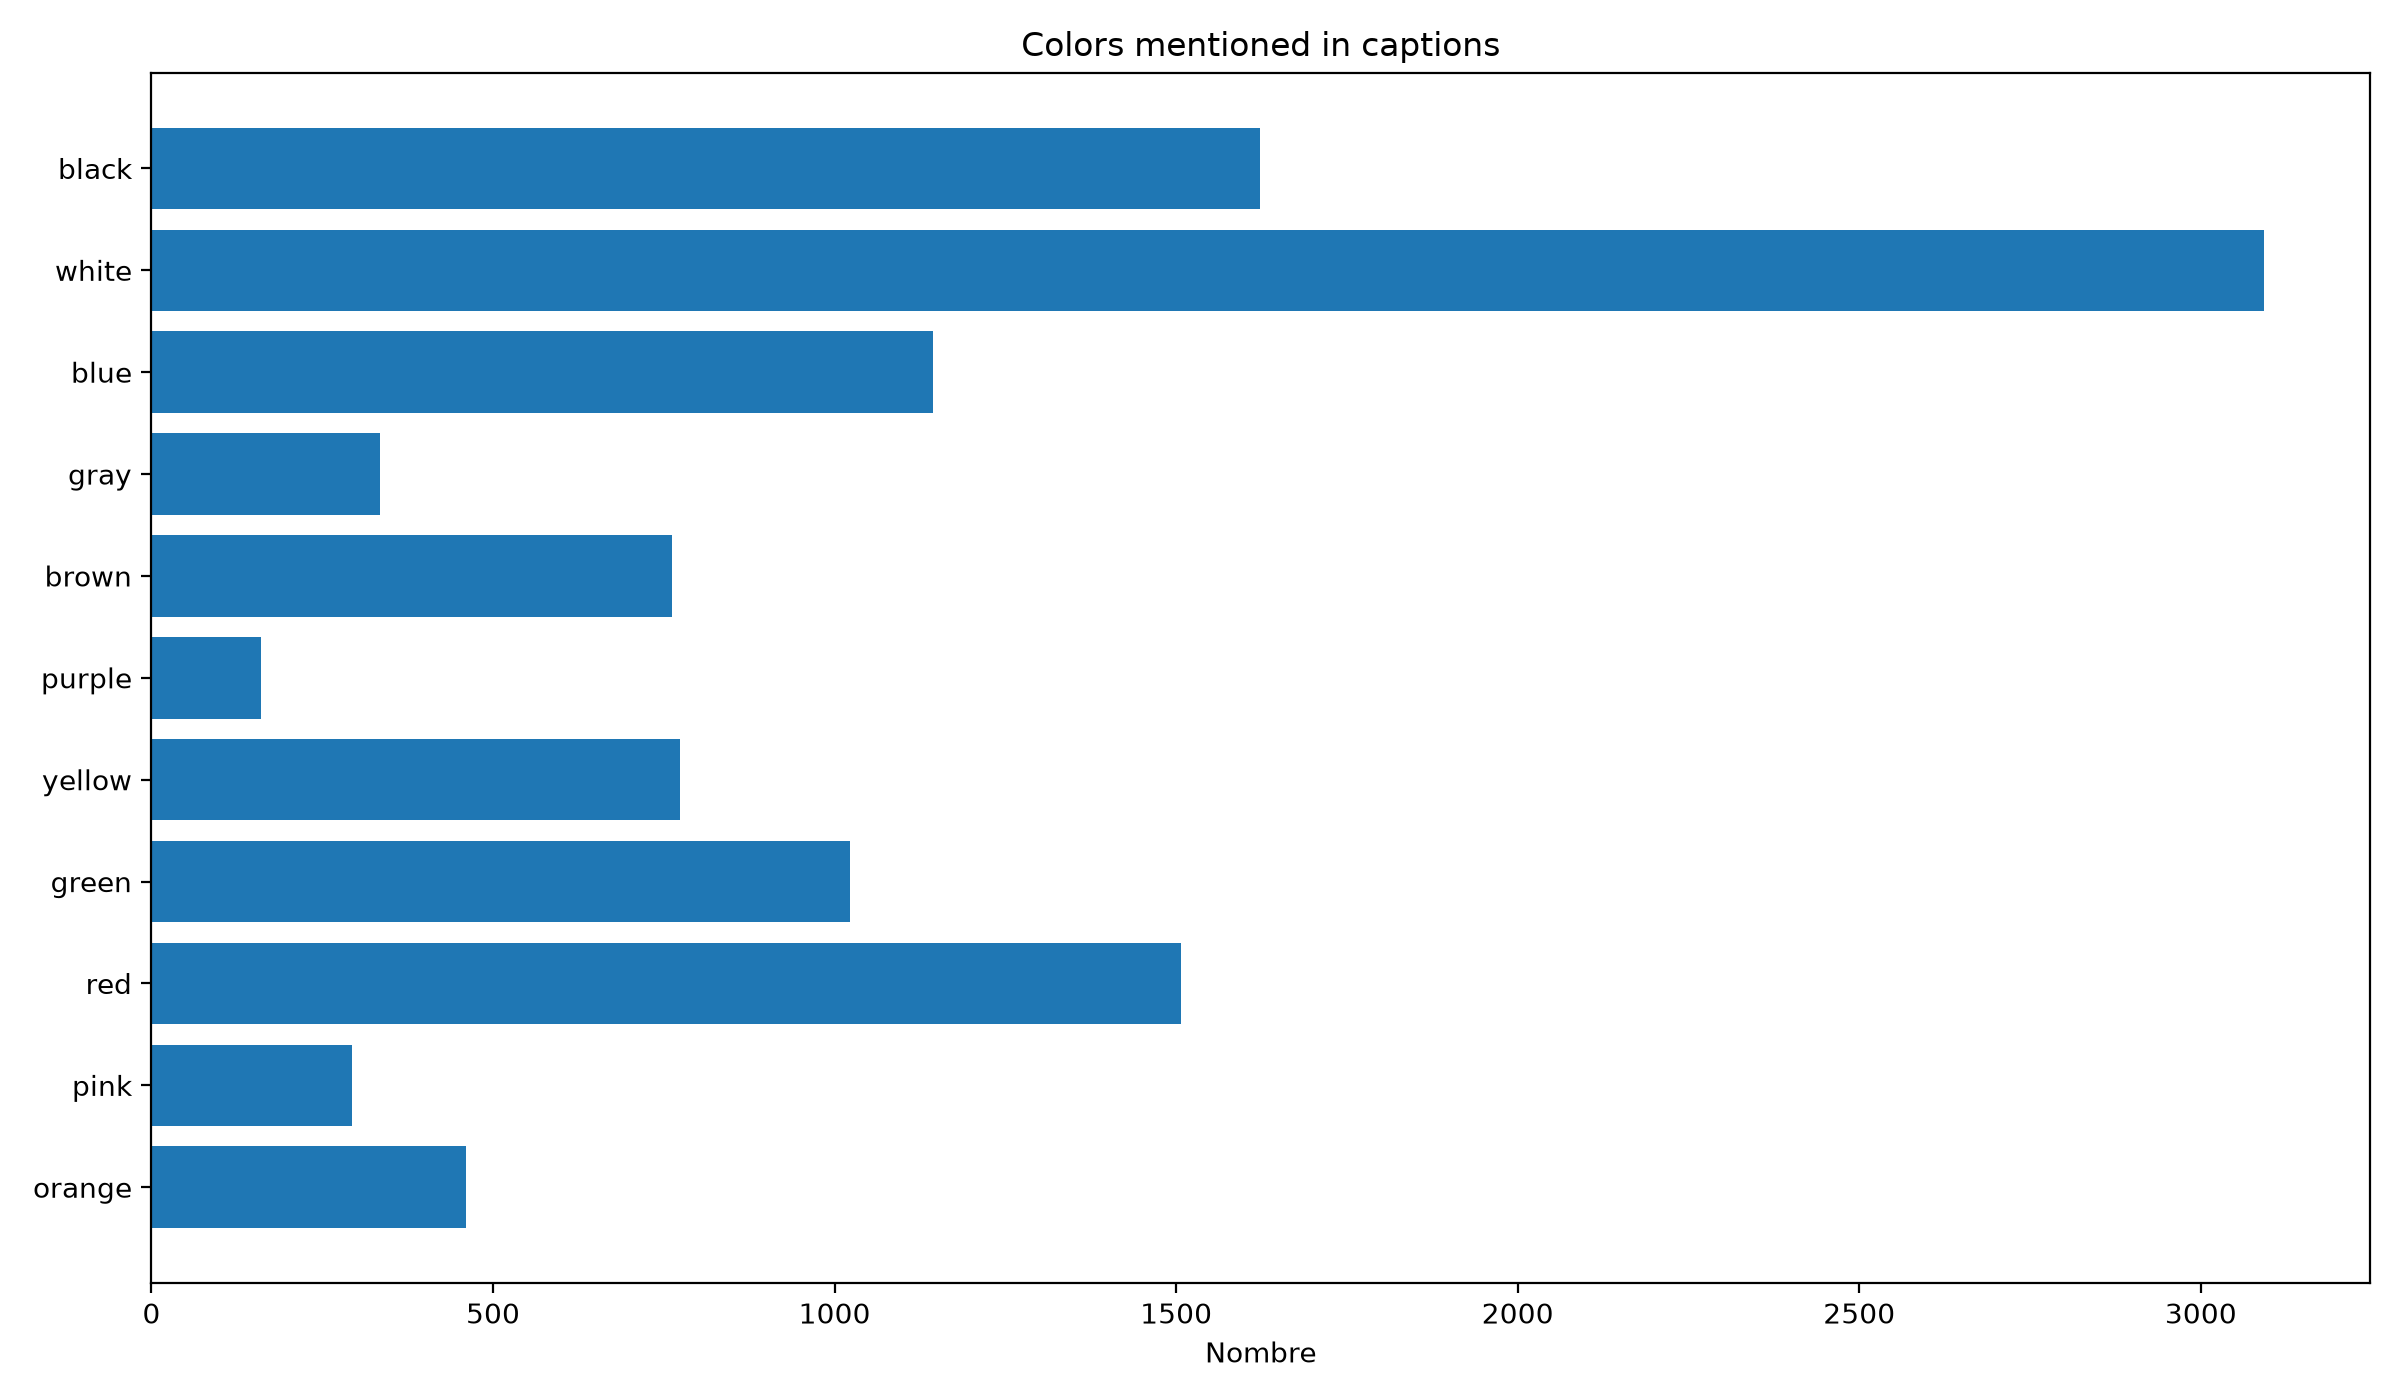
\includegraphics[width=0.48\textwidth]{figures/color_distribution.png}\hfill
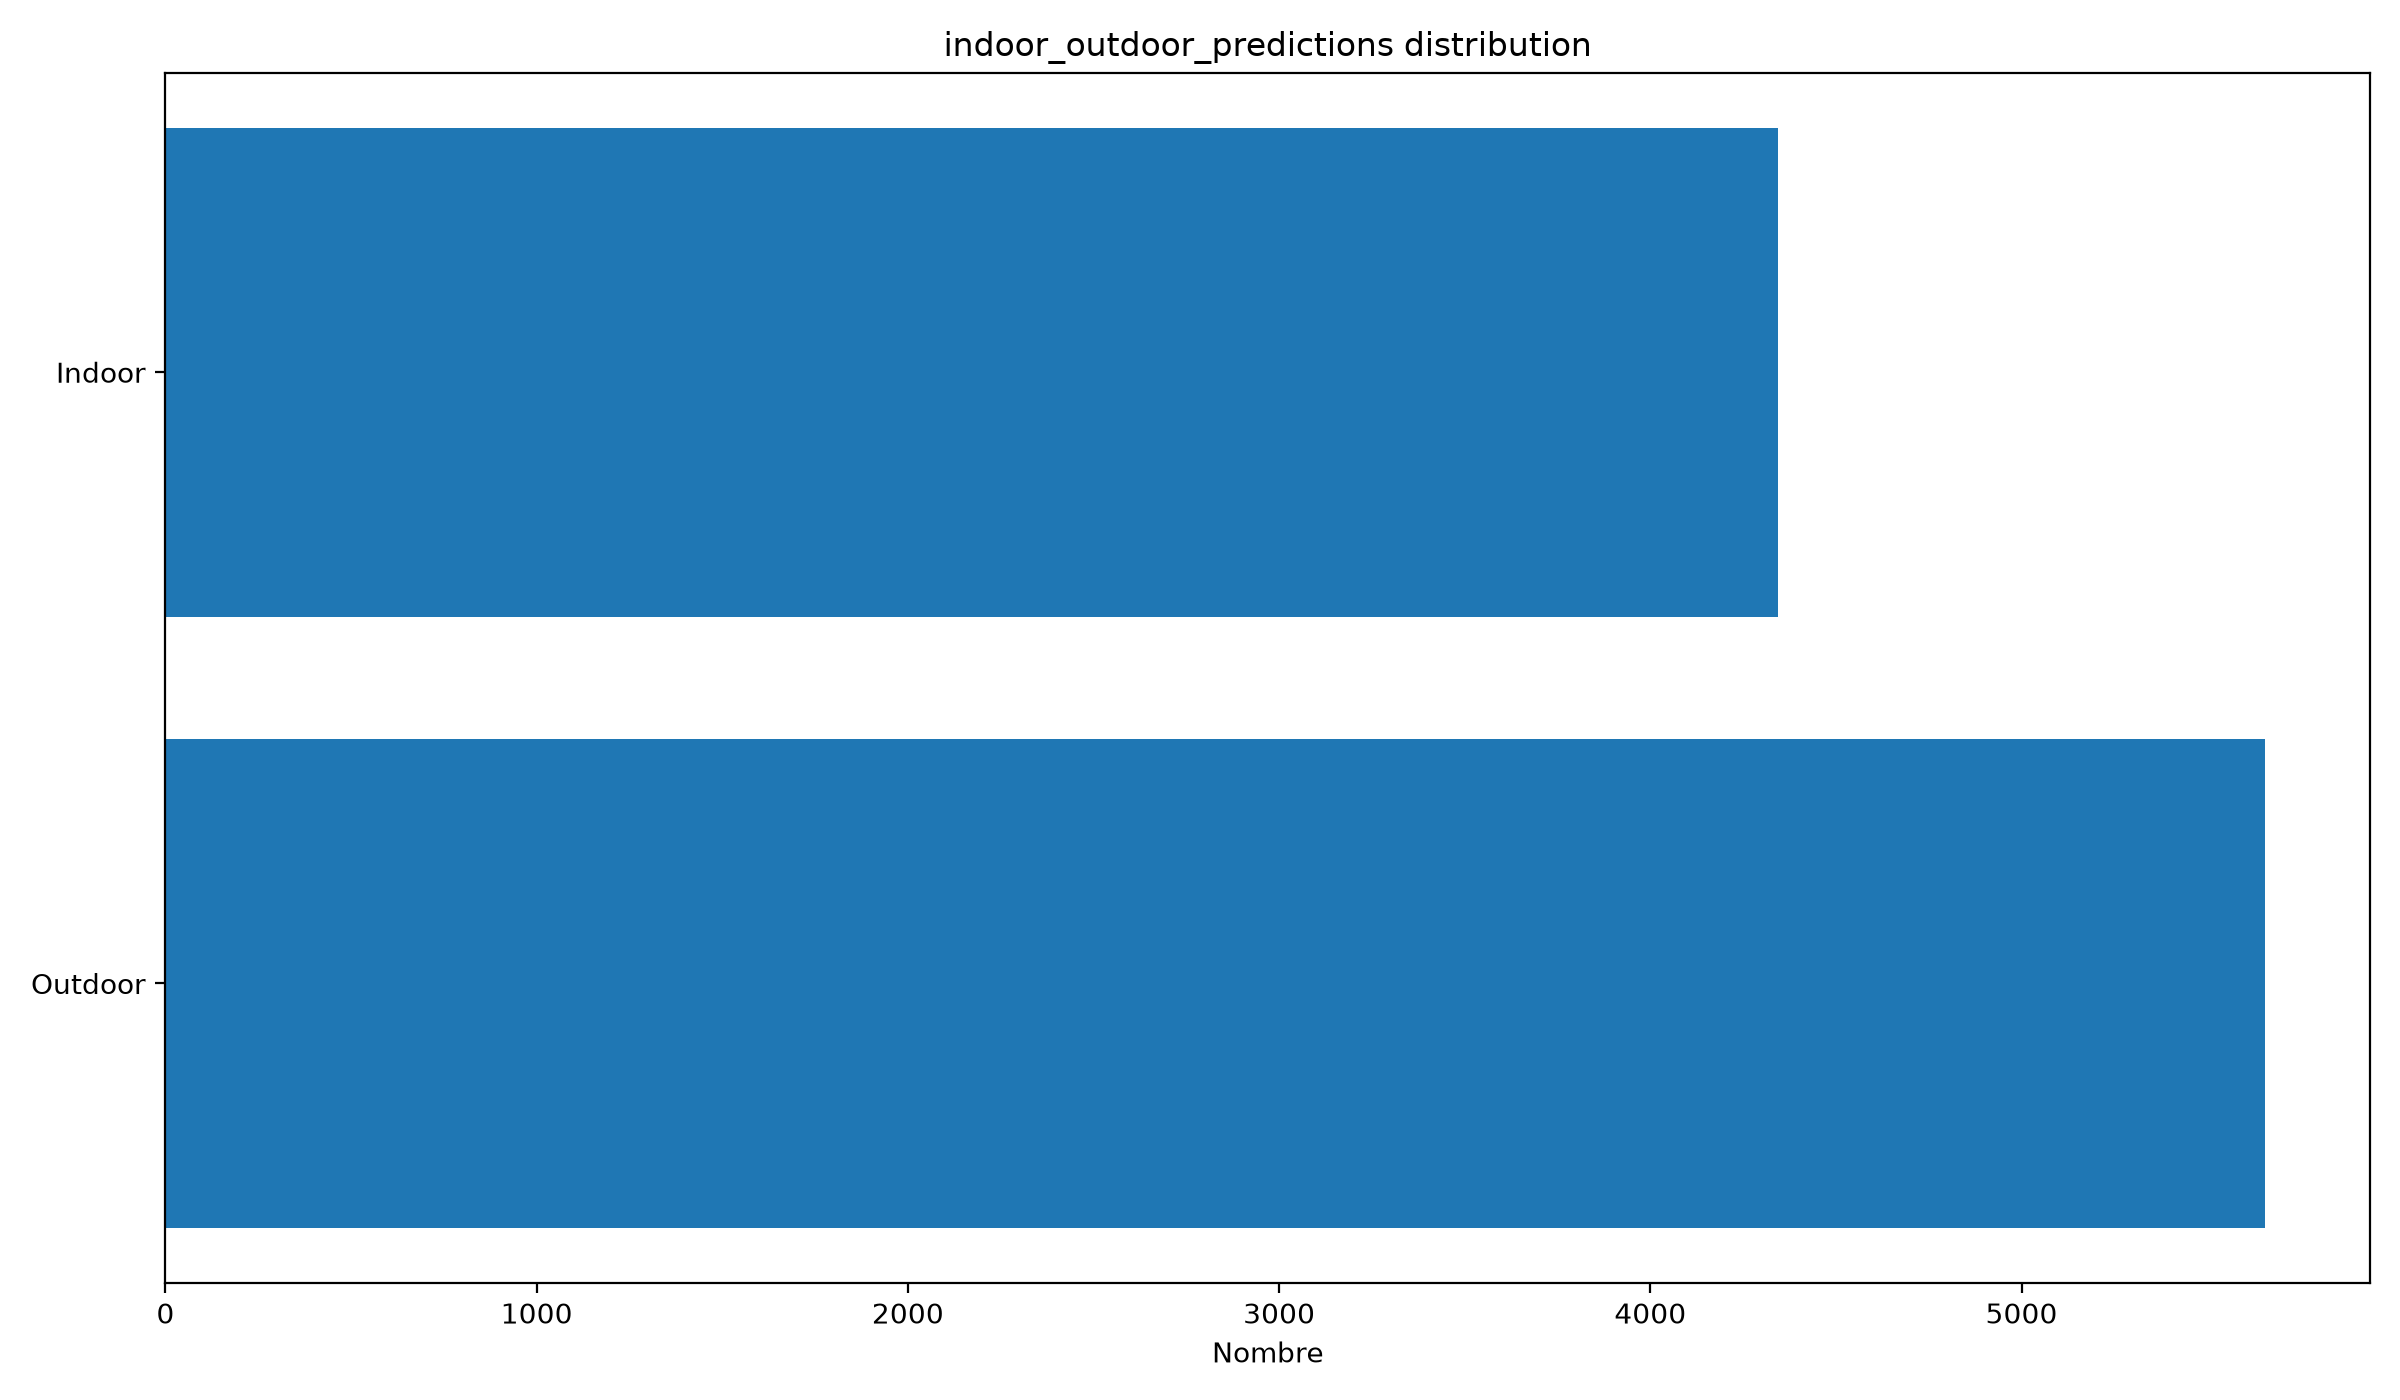
\includegraphics[width=0.48\textwidth]{figures/indoor_outdoor_distribution.png}\\[2mm]
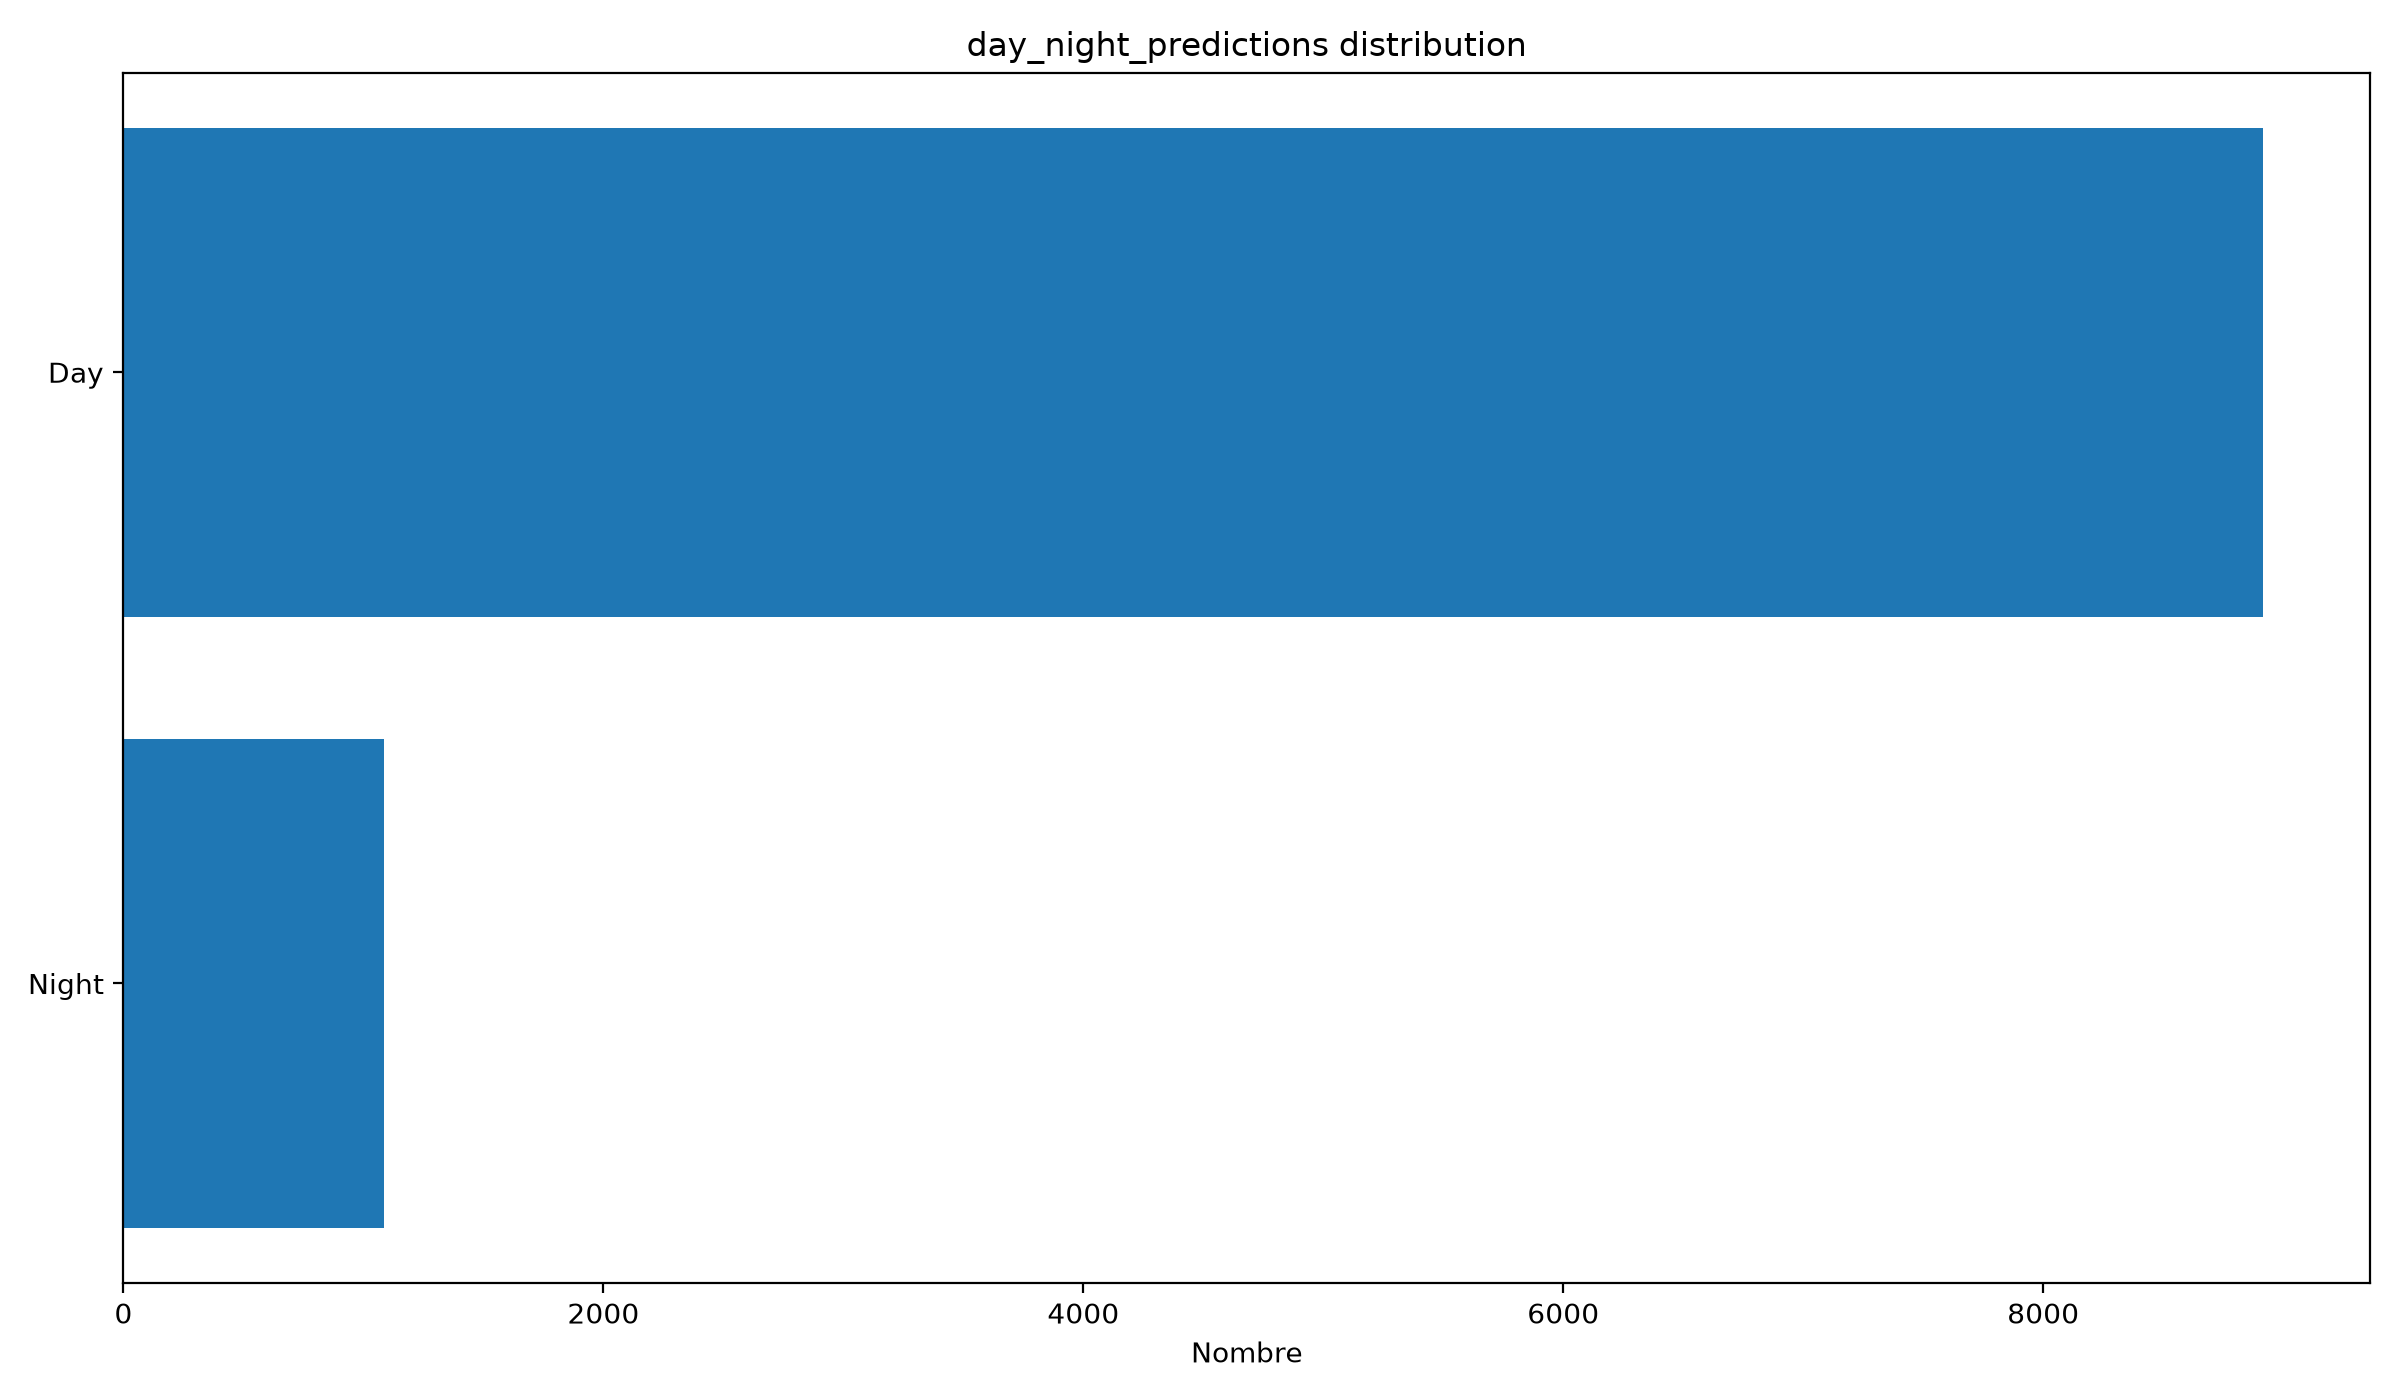
\includegraphics[width=0.48\textwidth]{figures/day_night_distribution.png}
\caption{Colours mentioned in captions (top left), CLIP indoor/outdoor prediction (top right) and CLIP day/night prediction (bottom).}
\label{fig:kbdiversity}
\end{figure}

\begin{interp}
\begin{itemize}[nosep]
  \item \textbf{Noun-centred captions.} Nouns are by far the most frequent tag (about 180\,000 tokens), followed by determiners (about 107\,000), adpositions (about 89\,000), verbs (about 51\,000) and adjectives (about 38\,000). This confirms the word-level findings of the previous section: captions name objects and place them with prepositions, so object and relation hallucinations are the natural errors to measure.
  \item \textbf{Colours.} \emph{White} is the most frequent colour word (about 3\,100 mentions), well ahead of \emph{black}, \emph{red}, \emph{blue} and \emph{green} (about 1\,000 to 1\,600 each); \emph{purple}, \emph{pink} and \emph{gray} are rare. Attribute hallucinations will be easier to measure for the frequent colours than for the rare ones.
  \item \textbf{Contexts.} CLIP predicts roughly 57\,\% outdoor and 43\,\% indoor images, and about 89\,\% day against 11\,\% night. Indoor and outdoor scenes are both well represented, but \textbf{night scenes are rare}: results on night images will rest on few examples and should not be over-interpreted.
  \item \textbf{Precision of these values.} The counts quoted in this subsection are read from the figures, hence the ``about''; the exact values are in the JSON files of \code{data/exploration/} (Git LFS).
\end{itemize}
\end{interp}

\subsection{Summary of the exploration}
\begin{table}[H]
\centering
\begin{tabular}{@{}p{5.2cm}p{9.5cm}@{}}
\toprule
\textbf{Property} & \textbf{Finding}\\
\midrule
Object classes & 80 classes, 860\,001 annotations; ``person'' = 30.5\,\%; top 50 = 88.8\,\%.\\
Scene complexity & 7.27 objects/image on average; strongly right-skewed, many simple scenes and a long tail of cluttered ones.\\
Captions & 10.48 words on average (median 10, range 5--50); 26\,466 distinct words.\\
Vocabulary & Dominated by function words (top 30 = 48.5\,\% of tokens); content centred on people, postures and locations.\\
Contexts & Balanced indoor and outdoor scenes (about 43\,\% / 57\,\% predicted by CLIP on the knowledge base); night scenes are rare (about 11\,\%).\\
Attributes & Colours mentioned in captions are dominated by \emph{white}; nouns dominate the POS distribution.\\
\bottomrule
\end{tabular}
\caption{Key exploration findings.}
\end{table}

%====================================================================
\section{Pre-processing steps}

\subsection{Step 2 --- Split creation and anti-leakage control}
\label{sec:splits}

\paragraph{Objective.} Create and freeze three disjoint splits (knowledge base, validation, test) and guarantee that no test reference caption can ever be retrieved or used (anti-leakage rule of Section~4.2).

\paragraph{Method (\code{create\_splits.py}).}
\begin{enumerate}[nosep]
  \item Load the image IDs of train2017 and val2017 and check that they are unique (an exception is raised otherwise).
  \item Check sizes: train2017 must contain at least $10\,000+100$ images, val2017 at least $N_{\text{test}}$.
  \item Set \code{random.seed(42)}, shuffle the train2017 IDs, take the first 10\,000 as the \textbf{knowledge base} and the next 100 (positions 10\,000--10\,099) as the \textbf{validation} set. Because the two slices of the same shuffled list cannot overlap, the validation images are disjoint from the knowledge base by construction.
  \item Shuffle the val2017 IDs and take the first 100 as the \textbf{test} set. Test images come from a \emph{different official split} than the knowledge base, so they cannot appear in it.
  \item Execute three \code{assert} statements verifying that the three ID sets are pairwise disjoint. 
  \item Save the three image-ID lists as JSON files in \code{data/splits/}: knowledge\_base\_image\_ids.json, validation\_image\_ids.json, and test\_image\_ids.json.
  \item \textbf{Test-set extension} (\code{create\_updated\_test\_split.py}): add 900 random val2017 images to the original 100 to obtain \code{test\_1000\_image\_ids.json}, and keep the original list as \code{test\_100\_image\_ids\_legacy.json} (see the remark of Section~3). \code{check\_current\_splits.py} re-verifies the provenance (knowledge base and validation in train2017, test in val2017) and the pairwise overlaps without modifying any file.
\end{enumerate}


\begin{table}[H]
\centering
\begin{tabular}{@{}lrr@{}}
\toprule
\textbf{Check} & \textbf{Value} & \textbf{Status}\\
\midrule
Knowledge-base images & 10\,000 & \texttt{PASS}\\
Validation images & 100 & \texttt{PASS}\\
Test images & 100 & \texttt{PASS}\\
Duplicate IDs inside each split & 0 / 0 / 0 & \texttt{PASS}\\
KB $\cap$ validation & 0 & \texttt{PASS}\\
KB $\cap$ test & 0 & \texttt{PASS}\\
Validation $\cap$ test & 0 & \texttt{PASS}\\
\bottomrule
\end{tabular}
\caption{Split verification (source: \code{quality\_control\_report.json}, run with the 100-image test file; to be re-run for \code{test\_1000\_image\_ids.json}).}
\end{table}

\begin{interp}
The two sampling strategies give two layers of protection: (i) \emph{ID disjointness} (verified by assertion, and again by the quality-control script), and (ii) \emph{source separation} (test images are drawn from val2017, the knowledge base from train2017). Moreover, only the captions of the 10\,000 knowledge-base images are ever loaded into the text index (Step~4), so \textbf{no test caption can be retrieved} -- the quality-control step checks this explicitly ($0$ test or validation IDs in the text embeddings). Fixing the seed makes the splits perfectly reproducible and identical for all 30 groups once the ID files are shared. For the extended test set, source separation (val2017 versus train2017) gives the same guarantee for the 900 added images, but the formal \code{quality\_control.py} audit has not yet been re-run on them.
\end{interp}


%--------------------------------------------------------------------
\subsection{Step 3 --- Image pre-processing}
\label{sec:images}

\paragraph{Objective.} Obtain, for the 10\,000 knowledge-base images, RGB images with a correct orientation, ready for the image encoder, while keeping the original aspect ratio.

\paragraph{Method (\code{preprocess\_images.py}).} For each ID of the knowledge base:
\begin{enumerate}[nosep]
  \item open \code{train2017/\{id:012d\}.jpg} and record the original width and height;
  \item apply \code{ImageOps.exif\_transpose} to correct the orientation stored in the EXIF metadata;
  \item convert to RGB mode (\code{convert("RGB")}) so that grey-scale or palette images have three channels;
  \item record the processed size and save the image as JPEG (quality 95) in \code{data/processed\_images/};
  \item catch any exception per image and log it in an \code{errors} list, so that one failure does not stop the process.
\end{enumerate}
\textbf{No resizing or cropping is performed in this script}: resizing and normalisation depend on the assigned image encoder, so they are delegated to the encoder's own processor (\code{CLIPProcessor}) in Step~6. For CLIP ViT-B/32 this processor resizes the shortest side to 224 pixels (bicubic), centre-crops to $224\times224$ and normalises with the CLIP channel means and standard deviations.


\begin{table}[H]
\centering
\small
\renewcommand{\arraystretch}{1.15}
\begin{tabularx}{\textwidth}{@{}>{\raggedright\arraybackslash}p{7.2cm} >{\raggedleft\arraybackslash}X@{}}
\toprule
\textbf{Indicator} & \textbf{Value}\\
\midrule
Images to process & 10\,000\\
Successful / failed & 10\,000 / 0\\
Colour mode after processing & RGB for 10\,000 images\\
Images whose size changed after EXIF correction & 0\\
Width: min / mean / max (px) & 150 / 579.3 / 640\\
Height: min / mean / max (px) & 120 / 483.3 / 640\\
Mean aspect ratio (width/height) & 1.26\\
Landscape / portrait / square images & 7\,352 / 2\,306 / 342\\
Most frequent size & $640\times480$ (2\,208 images, 22.1\,\%)\\
Other frequent sizes & $640\times427$ (1\,246), $480\times640$ (733), $640\times426$ (473), $500\times375$ (447)\\
\bottomrule
\end{tabularx}
\caption{Image pre-processing results (source: \code{image\_preprocessing\_report.json}, computed over the 10\,000 images).}
\label{tab:image-preprocessing}
\end{table}

\begin{figure}[H]
\centering
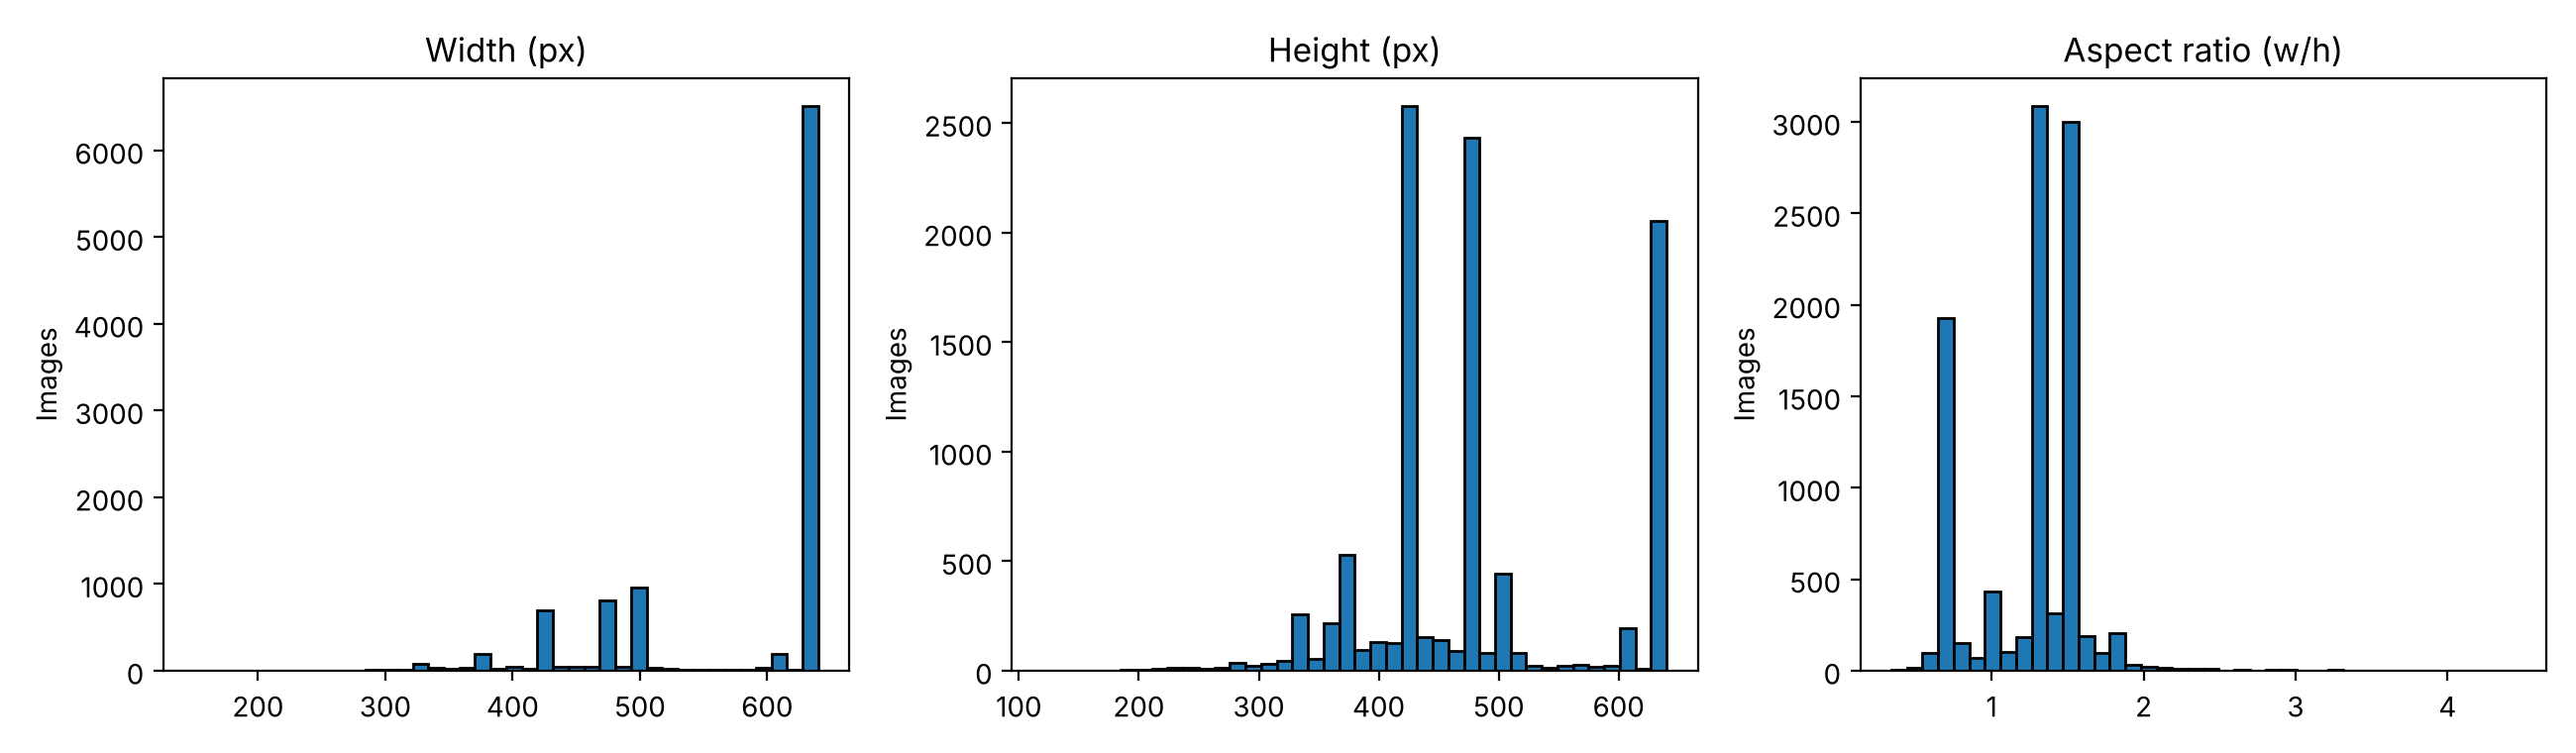
\includegraphics[width=\textwidth]{figures/kb_image_sizes.png}
\caption{Distribution of width, height and aspect ratio of the 10\,000 knowledge-base images.}
\label{fig:imgsizes}
\end{figure}

\begin{interp}
\begin{itemize}[nosep]
  \item \textbf{100\,\% success, no information loss in geometry.} No image failed, all are RGB, and none changed size after the EXIF transposition: none of these 10\,000 images carried a rotation tag that changes its dimensions, so this operation acts as a safeguard rather than a correction. The pipeline is nevertheless robust to datasets that do.
  \item \textbf{Heterogeneous formats.} COCO images have at most 640 pixels on the long side, with typical sizes $640\times480$ or $640\times427$. About 73.5\,\% of the images are landscape, 23.1\,\% portrait and 3.4\,\% square. Because CLIP centre-crops to a square, \textbf{the left/right borders of landscape images are cut off} (about 25\,\% of the width for a $4{:}3$ image). Objects located near the borders may therefore be invisible to the encoder; this is a known limitation of CLIP-based retrieval and a possible cause of omissions.
  \item \textbf{Low resolution of the source.} The images are small (579$\times$483 on average), so the processed JPEGs are already below the native resolution that modern VLMs use; this limits the visibility of small objects, which are the most frequently hallucinated or omitted ones.
  \item \textbf{Re-encoding.} Saving at JPEG quality 95 introduces a tiny additional compression artefact relative to the original files. It is imperceptible for the encoder but should be mentioned for strict reproducibility.
\end{itemize}
\end{interp}

%--------------------------------------------------------------------
\subsection{Step 4 --- Caption pre-processing}
\label{sec:captions}

\paragraph{Objective.} Provide both the \emph{raw} reference captions (unchanged, used for evaluation) and a \emph{cleaned} version used only for retrieval and indexing, stored with distinct field and file names to avoid evaluation leakage.

\paragraph{Method (\code{preprocess\_captions.py}).}
\begin{enumerate}[nosep]
  \item Load \code{captions\_train2017.json} and the knowledge-base IDs.
  \item Keep only the annotations whose \code{image\_id} belongs to the knowledge base (a set lookup, $O(1)$ per annotation).
  \item For each kept annotation, store the \textbf{raw} caption unchanged (\code{kb\_captions\_raw.json}) and a \textbf{cleaned} caption (\code{kb\_captions\_cleaned.json}), both keeping \code{annotation\_id} and \code{image\_id}.
  \item The cleaning function applies: (a) lower-casing, (b) stripping leading/trailing spaces, (c) collapsing multiple whitespace characters (\verb|\s+| $\to$ single space), (d) removing spaces before punctuation (\verb|\s+([.,!?;:])|).
  \item Validate: every knowledge-base image has captions, the number of captions per image is reported, and the raw and cleaned lists have the same length.
\end{enumerate}
Punctuation is \emph{not} removed, and no explicit tokenisation is stored: tokenisation is left to the encoder (CLIP's byte-pair-encoding tokenizer, which handles punctuation by itself) and to the sparse retrievers assigned to some groups.

\begin{table}[H]
\centering
\begin{tabular}{@{}lr@{}}
\toprule
\textbf{Indicator} & \textbf{Value}\\
\midrule
Knowledge-base images & 10\,000\\
Raw captions / cleaned captions & 50\,028 / 50\,028\\
Images without captions & 0\\
Images with exactly 5 captions & 9\,972\\
Images with 6 captions & 28\\
Images with fewer than 5 captions & 0\\
Raw and cleaned counts match & \texttt{True}\\
\bottomrule
\end{tabular}
\caption{Caption pre-processing (source: \code{caption\_preprocessing\_report.json}).}
\end{table}

\begin{interp}
\begin{itemize}[nosep]
  \item \textbf{50\,028 instead of 50\,000 captions.} 28 knowledge-base images have 6 captions ($28$ extra captions), in agreement with the audit ($0.28\,\%$ of the images, a proportion close to the $0.27\,\%$ observed in the full train2017 set, i.e. $315/118\,287$). We keep all of them: the extra captions are valid human references, and removing them would require an arbitrary choice.
  \item \textbf{Evaluation integrity.} Because cleaning (lower-casing etc.) can change n-gram matches in BLEU/CIDEr, the evaluation must always use the raw captions, while retrieval uses the cleaned ones. Keeping two files with identical IDs makes this separation explicit and prevents accidental mixing.
  \item \textbf{Minimal cleaning is intentional.} Over-aggressive cleaning (stop-word removal, stemming) would damage dense embeddings, which are trained on natural sentences. The cleaning only removes formatting noise (case, spaces), so the semantics are preserved.
  \item \textbf{Alignment.} The same \code{annotation\_id} appears in both versions, so each cleaned caption can be traced back to its raw original.
\end{itemize}
\end{interp}

%--------------------------------------------------------------------
\subsection{Step 5 --- Metadata extraction}
\label{sec:metadata}

\paragraph{Objective.} Attach to each knowledge-base image its visual metadata: detected objects, scene information and spatial relations, so that the metadata-filtered and multimodal RAG groups can use them.

\paragraph{Method (\code{extract\_metadata.py}).} Instead of running an object detector, the script uses the \textbf{ground-truth COCO instance annotations} (\code{instances\_train2017.json}), which are permitted as ``annotation fields'' by the statement (Section~4.4.3, step 5). For every knowledge-base image it stores:
\begin{itemize}[nosep]
  \item image information: file name, width, height;
  \item the raw captions of the image;
  \item the list of objects: \code{annotation\_id}, \code{category\_id}, category name, \code{bbox} ($[x,y,w,h]$), \code{area}, \code{iscrowd};
  \item \code{object\_count};
  \item \textbf{spatial relations} between every pair of objects.
\end{itemize}

\paragraph{Spatial relation rule.} For two objects $A$ and $B$ with boxes $(x,y,w,h)$, the centres are $c_A=(x_A+w_A/2,\;y_A+h_A/2)$ and $c_B$. The relations are
\begin{align*}
&\text{left\_of if } c_{A,x}<c_{B,x}, \qquad \text{right\_of if } c_{A,x}>c_{B,x},\\
&\text{above if } c_{A,y}<c_{B,y}, \qquad \text{below if } c_{A,y}>c_{B,y},
\end{align*}
so each pair yields up to two relations (one horizontal and one vertical). Results are saved as \code{kb\_metadata.json}, a per-image summary \code{kb\_metadata\_summary.csv} (image ID, file name, size, object count, caption count, number of relations) and a global statistics file \code{metadata\_statistics.json} (total objects, mean objects per image, relation-type counts, category counts).

\paragraph{Optional detector branch (YOLO).} The statement lists an object detector as optional. In addition to the ground-truth annotations, a YOLO detector (\code{yolo26n.pt}, confidence threshold 0.25, CPU) was run on the knowledge-base images, in four stages: a 100-image pilot (\code{pilot\_yolo\_100.py}, evaluated by \code{evaluate\_yolo\_pilot\_100.py}); a threshold experiment over $\{0.25,0.40,0.50\}$ with an IoU threshold of 0.50 (\code{experiment\_yolo\_thresholds.py}, \code{compare\_yolo\_coco.py}); the full extraction on the 10\,000 images (\code{extract\_yolo\_10000.py}, checkpoint every 100 images); and the merge with the COCO metadata (\code{merge\_yolo\_metadata.py}). The merged file \code{kb\_metadata\_with\_yolo.json} adds three fields to each image (\code{yolo\_detections}, \code{yolo\_detection\_count}, \code{yolo\_detected\_categories}) and preserves the COCO fields. SHA-256 checksums of inputs and outputs are stored in \code{reports/yolo\_merge\_sha256.json}. The merged file and the weights are excluded from Git (\code{.gitignore}) because of their size and are regenerated by the scripts.

\begin{table}[H]
\centering
\begin{tabular}{@{}lr@{}}
\toprule
\textbf{Indicator} (source: \code{yolo\_metadata\_merge\_report.json}) & \textbf{Value}\\
\midrule
Model / threshold / device & \code{yolo26n.pt} / 0.25 / CPU\\
Images merged (unique image IDs) & 10\,000\\
Total detections & 49\,375\\
Mean detections per image & 4.94\\
Detected categories (out of 80) & 79\\
Images without any detection & 136 (1.4\,\%)\\
Merge quality-control flags (7) & all \code{true}\\
\bottomrule
\end{tabular}
\caption{Merge of the YOLO detections with the COCO metadata.}
\end{table}

\begin{remark}[Two bounding-box conventions]
COCO boxes are stored as $[x,y,w,h]$, YOLO boxes as $[x_1,y_1,x_2,y_2]$: any group that uses both sources must convert one convention to the other. YOLO detections are \emph{predicted} objects and contain detection errors, unlike the COCO annotations: they are the realistic query-time source for the metadata-filtered groups (G28--G30), whereas the COCO annotations remain the oracle.
\end{remark}

\begin{interp}
\begin{itemize}[nosep]
  \item \textbf{Ground truth as the primary source.} COCO annotations are human-verified, so this metadata has no detection noise, no confidence threshold to tune and no model version to document. This provides an \emph{upper bound} (an ``oracle'') for metadata-based techniques; it also gives the reference needed to measure object hallucination later (is a generated object in the annotated list?).
  \item \textbf{Expected content.} Since the 10\,000 images are a uniform random sample of train2017, their metadata should reflect the exploration of Section~\ref{sec:explore}: about 7.3 objects per image and about 30\,\% of them persons.
  \item \textbf{Number of relations grows quadratically.} For an image with $n$ objects, $\binom{n}{2}$ pairs and up to $2\binom{n}{2}$ relations are stored. A cluttered image with 90 objects yields several thousand relations, which is why the full metadata file is large and why this representation should be filtered (e.g. to the biggest or non-crowd objects) before being injected into a prompt.
  \item \textbf{Limits of the relation rule.} Comparing box centres is a coarse approximation: it does not capture ``on'', ``next to'', ``in front of'' or containment, and an object can be simultaneously ``left\_of'' and ``above'' another one. These are \emph{geometric} relations in the image plane, not semantic relations as expressed in captions.
  \item \textbf{Attributes.} COCO provides no attribute annotations (colour, material), so the ``attributes'' field requested by the statement is not populated by this script; attribute information can only come from the captions or from a separate model.
\end{itemize}
\end{interp}



%--------------------------------------------------------------------


\subsection{Step 6 --- Embedding generation}
\label{sec:embeddings}

\paragraph{Objective.} Encode every knowledge-base image and every cleaned caption into a common vector space, so that image-to-image, image-to-text, text-to-image and text-to-text retrieval are all possible.

\paragraph{Model choice.} \textbf{CLIP ViT-B/32}~\cite{clip} (\code{openai/clip-vit-base-patch32}, Hugging Face Transformers) is used as image encoder \emph{and} text encoder. CLIP is trained contrastively so that matching image/text pairs have a high cosine similarity; this makes cross-modal retrieval possible with a single model and a single index dimension (512). It is one of the image encoders allowed by the statement (CLIP, SigLIP, DINOv2) and has the lowest computational cost of the CLIP family, an advantage on CPU-only hardware.

\paragraph{Method (\code{generate\_embeddings.py}).}
\begin{enumerate}[nosep]
  \item Load the knowledge-base IDs and the \textbf{cleaned} captions, keeping only captions of knowledge-base images; stop if an image has no caption or a processed image file is missing.
  \item \textbf{Image embeddings}: batches of 32 images are converted by \code{CLIPProcessor}, passed through the vision transformer (\code{vision\_model}, pooled output) and the visual projection layer; the 512-d vector is \textbf{L2-normalised}.
  \item \textbf{Text embeddings}: batches of 32 captions are tokenised (padding, truncation to 77 tokens), passed through the text transformer and the text projection; the 512-d vector is \textbf{L2-normalised}.
  \item Everything is computed under \code{torch.no\_grad()} in evaluation mode; the device is chosen automatically (CUDA if available, otherwise CPU).
  \item Save \code{image\_embeddings.npy}, \code{text\_embeddings.npy} and three ID arrays (\code{image\_ids}, \code{text\_image\_ids}, \code{text\_annotation\_ids}) that link every row to its image/caption, together with \code{embedding\_metadata.json} (model, dimension, counts, batch size, normalisation flags).
\end{enumerate}

\begin{table}[H]
\centering
\begin{tabular}{@{}lr@{}}
\toprule
\textbf{Property} & \textbf{Value}\\
\midrule
Model & \code{openai/clip-vit-base-patch32}\\
Embedding dimension & 512\\
Image embeddings & $10\,000\times512$, \code{float32}\\
Text embeddings & $50\,028\times512$, \code{float32}\\
Batch size & 32\\
Max text length & 77 tokens\\
Normalisation & L2 (unit norm) for images and texts\\
Memory (images) & $10\,000\times512\times4$ B $\approx$ 19.5 MiB\\
Memory (texts) & $50\,028\times512\times4$ B $\approx$ 97.7 MiB\\
\bottomrule
\end{tabular}
\caption{Embedding configuration and sizes (sources: \code{embedding\_metadata.json}, \code{quality\_control\_report.json}).}
\end{table}

\begin{interp}
\begin{itemize}[nosep]
  \item \textbf{Why L2 normalisation.} After normalisation, the inner product equals the cosine similarity. This makes the similarity scores bounded in $[-1,1]$, independent of vector norms, and allows the use of a fast inner-product index.
  \item \textbf{A shared space.} Because images and texts live in the same 512-d space, the \emph{multimodal RAG} groups can retrieve captions with an image query, while the \emph{dense RAG} groups can embed a textual query and search images or captions without re-encoding the knowledge base. All groups share this single encoder, so differences between techniques are not caused by different embeddings.
  \item \textbf{Image/text asymmetry.} There are five times more text vectors than image vectors (50\,028 vs 10\,000), since each image has about five captions. Text vectors therefore carry the dominant share of the memory and of the search cost.
  \item \textbf{Variants for ablations.} Ablation~5 of the statement (CLIP vs SigLIP vs DINOv2) and the embedding-model hyper-parameter will require regenerating these files with another encoder; the script's \code{MODEL\_NAME} constant isolates this change.
\end{itemize}
\end{interp}

%--------------------------------------------------------------------

\subsection{Step 7 --- Knowledge-base construction}
\label{sec:kb}

\paragraph{Objective.} Build the vector databases on which all retrieval techniques will operate, and document the required elements: index type, similarity metric, dimension, size and a link between each vector and its image ID, captions and metadata.

\paragraph{Method (\code{build\_knowledge\_base.py}).}
\begin{enumerate}[nosep]
  \item Load the five embedding files and \textbf{validate} them: 2-D arrays, dimension 512, equal lengths between vectors and IDs, unique image IDs, absence of NaN/Inf, and every caption's image ID belongs to the knowledge base.
  \item Re-normalise the vectors (\code{faiss.normalize\_L2}) as a safety measure and cast them to contiguous \code{float32} arrays.
  \item Build \textbf{two FAISS indexes}: an image index and a text (caption) index, both of type \code{IndexFlatIP}.
  \item \raggedright Save the indexes and the ID mapping files (\code{image\_index\_ids.npy}, \code{text\_index\_image\_ids.npy}, \code{text\_index\_annotation\_ids.npy}) and the descriptor \code{knowledge\_base\_metadata.json}.
  \item Reload the indexes from disk and check that the number of stored vectors is unchanged.
\end{enumerate}

\begin{table}[H]
\centering
\begin{tabular}{@{}lp{9cm}@{}}
\toprule
\textbf{Documented item} & \textbf{Value}\\
\midrule
Library & FAISS~\cite{faiss} 1.15.1\\
Index type & \code{IndexFlatIP} (flat, exhaustive search, no compression)\\
Similarity metric & Inner product $=$ cosine similarity (normalised vectors)\\
Embedding dimension & 512\\
Image index size & 10\,000 vectors\\
Text index size & 50\,028 vectors\\
Row $\to$ record link & Row $i$ of the image index $\to$ \code{image\_index\_ids[i]}; row $j$ of the text index $\to$ \code{text\_index\_image\_ids[j]} and \code{text\_index\_annotation\_ids[j]}; metadata through the image ID.\\
\bottomrule
\end{tabular}
\caption{Knowledge-base documentation.}
\end{table}

\begin{interp}
\begin{itemize}[nosep]
  \item \textbf{Why a flat index.} With 10\,000 images and 50\,028 captions, an exhaustive search costs at most $50\,028\times512\approx2.6\times10^7$ multiply-adds per query, which is negligible (milliseconds). Approximate indexes (IVF, HNSW) would add training/hyper-parameter complexity and \emph{approximation error} without any benefit at this scale. The flat index returns the exact nearest neighbours, so retrieval quality is not confounded by index approximation, which is essential for a fair comparison of RAG techniques and for measuring retrieval latency.
  \item \textbf{Inner product $=$ cosine.} The \code{IndexFlatIP} on unit vectors ranks identically to a cosine-similarity search.
  \item \textbf{Separate image and text indexes.} They allow the four retrieval directions (I$\to$I, I$\to$T, T$\to$I, T$\to$T) needed by naive/dense, multimodal and hybrid RAG; the ID mapping converts any caption hit to its parent image, and vice versa.
  \item \textbf{Documentation gap.} The statement also requires the \emph{indexing time}. The script prints the execution time on the console but does not save it to a report; for a flat index this is a few seconds, since no training is needed and the vectors are only copied into the structure.
\end{itemize}
\end{interp}

%--------------------------------------------------------------------
\subsection{Step 8 --- Quality control}
\label{sec:qc}

\paragraph{Objective.} Detect missing embeddings, NaN values, duplicate IDs, caption mismatches and any data leakage before freezing the data.

\paragraph{Method (\code{quality\_control.py}).} The script performs ten independent checks, each recorded as \texttt{PASS}, \texttt{WARNING} or \texttt{FAIL} in \code{quality\_control\_report.json}:
\begin{enumerate}[nosep]
  \item \textbf{Splits}: sizes, duplicates inside each split, pairwise overlaps.
  \item \textbf{Embedding files}: all five files exist.
  \item \textbf{Embedding dimensions and types}: shapes $(10\,000,512)$ and $(50\,028,512)$, \code{float32}.
  \item \textbf{NaN / infinite values}: none in image or text embeddings.
  \item \textbf{Duplicate IDs}: image IDs and annotation IDs are unique.
  \item \textbf{L2 normalisation}: minimum and maximum vector norms are within a tolerance of 1.
  \item \textbf{Caption--image matching}: every caption points to a known image, every image has captions and embeddings, minimum/maximum captions per image.
  \item \textbf{Processed images}: the 10\,000 expected files exist.
  \item \textbf{FAISS indexes}: vector counts and dimensions are as expected.
  \item \textbf{Data leakage}: no overlap between splits and no validation/test image ID among the text-embedding image IDs.
\end{enumerate}

\begin{table}[H]
\centering
\small
\begin{tabular}{@{}llp{7.8cm}@{}}
\toprule
\textbf{Check} & \textbf{Status} & \textbf{Key values}\\
\midrule
Data splits & PASS & 10\,000 / 100 / 100 images; 0 duplicate; 0 overlap\\
Embedding files & PASS & 5 files found\\
Embedding dimensions & PASS & image $(10\,000,512)$; text $(50\,028,512)$; \code{float32}\\
NaN and infinite values & PASS & 0 invalid values (images and texts)\\
Duplicate IDs & PASS & 0 duplicate image IDs; 0 duplicate annotation IDs\\
L2 normalisation & PASS & norms in $[0.9999998,\,1.0000002]$ (images and texts)\\
Caption--image matching & PASS & 50\,028 captions; 10\,000 images with captions; captions per image: min 5, max 6; no missing/unknown\\
Processed images & PASS & 10\,000 expected, 0 missing\\
FAISS indexes & PASS & 10\,000 and 50\,028 vectors; $d=512$\\
Data leakage & PASS & 0 / 0 / 0 overlaps; 0 validation/test IDs in text embeddings\\
\midrule
\textbf{Overall} & \textbf{PASS} & 10 checks: 10 passed, 0 failed, 0 warnings, 0 errors\\
\bottomrule
\end{tabular}
\caption{Quality-control report.}
\label{tab:qc}
\end{table}

\begin{interp}
All ten checks pass with no warning. The normalisation deviation ($\le 2.4\times10^{-7}$) is pure \code{float32} rounding. The caption statistics (9\,972 images with 5 captions and 28 with 6) are consistent with the audit, the caption pre-processing report and the number of text vectors, which shows that the three representations (JSON, embeddings, index) have \textbf{consistent sizes}; the checks on IDs and the ID-mapping files then ensure that they are linked row by row. The leakage check is the most important: it confirms that the validation and test images are neither in the knowledge base nor in the text index, so evaluation on them is not biased by retrieval of their own captions.
\end{interp}

%--------------------------------------------------------------------
\subsection{Sanity validation with the retrieval pipeline}
\label{sec:retrieval}

\paragraph{Objective.} Section~4.4.4 requires that the frozen release \emph{works with the retrieval pipeline}. A dedicated script (\code{validate\_retrieval.py}) queries the knowledge base with the 100 \textbf{validation} images and their 500 captions, which are not in the knowledge base.

\paragraph{Method.} The validation images are loaded from train2017 (EXIF-corrected, RGB), encoded with the same CLIP model and normalisation, and searched with $k=10$ (CPU, batch size 16) in four configurations:
\begin{center}
\small
\begin{tabular}{@{}lll@{}}
\toprule
\textbf{Experiment} & \textbf{Queries} & \textbf{Searched index}\\
\midrule
Image $\to$ Image & 100 images & image index\\
Image $\to$ Text & 100 images & text (caption) index\\
Text $\to$ Image & 500 captions & image index\\
Text $\to$ Text & 500 captions & text index\\
\bottomrule
\end{tabular}
\end{center}
For each query, the ten best IDs and their cosine similarities are saved in \code{image\_retrieval\_results.json} and \code{caption\_retrieval\_results.json}. As the script itself states, no relevance judgements are available, so these results are \emph{rankings and similarity scores}, not precision/recall.

\paragraph{Results.} Mean, minimum and maximum of the \textbf{top-1 cosine similarity} per experiment:
\begin{table}[H]
\centering
\begin{tabular}{@{}lrrrr@{}}
\toprule
\textbf{Experiment} & \textbf{Queries} & \textbf{Mean top-1} & \textbf{Min} & \textbf{Max}\\
\midrule
Image $\to$ Image & 100 & 0.814 & 0.579 & 0.946\\
Image $\to$ Text & 100 & 0.328 & 0.283 & 0.391\\
Text $\to$ Image & 500 & 0.325 & 0.237 & 0.393\\
Text $\to$ Text & 500 & 0.889 & 0.565 & 1.000\\
\bottomrule
\end{tabular}
\caption{Top-1 similarity statistics of the validation retrieval (computed from the result files).}
\label{tab:retr}
\end{table}

\begin{figure}[H]
\centering
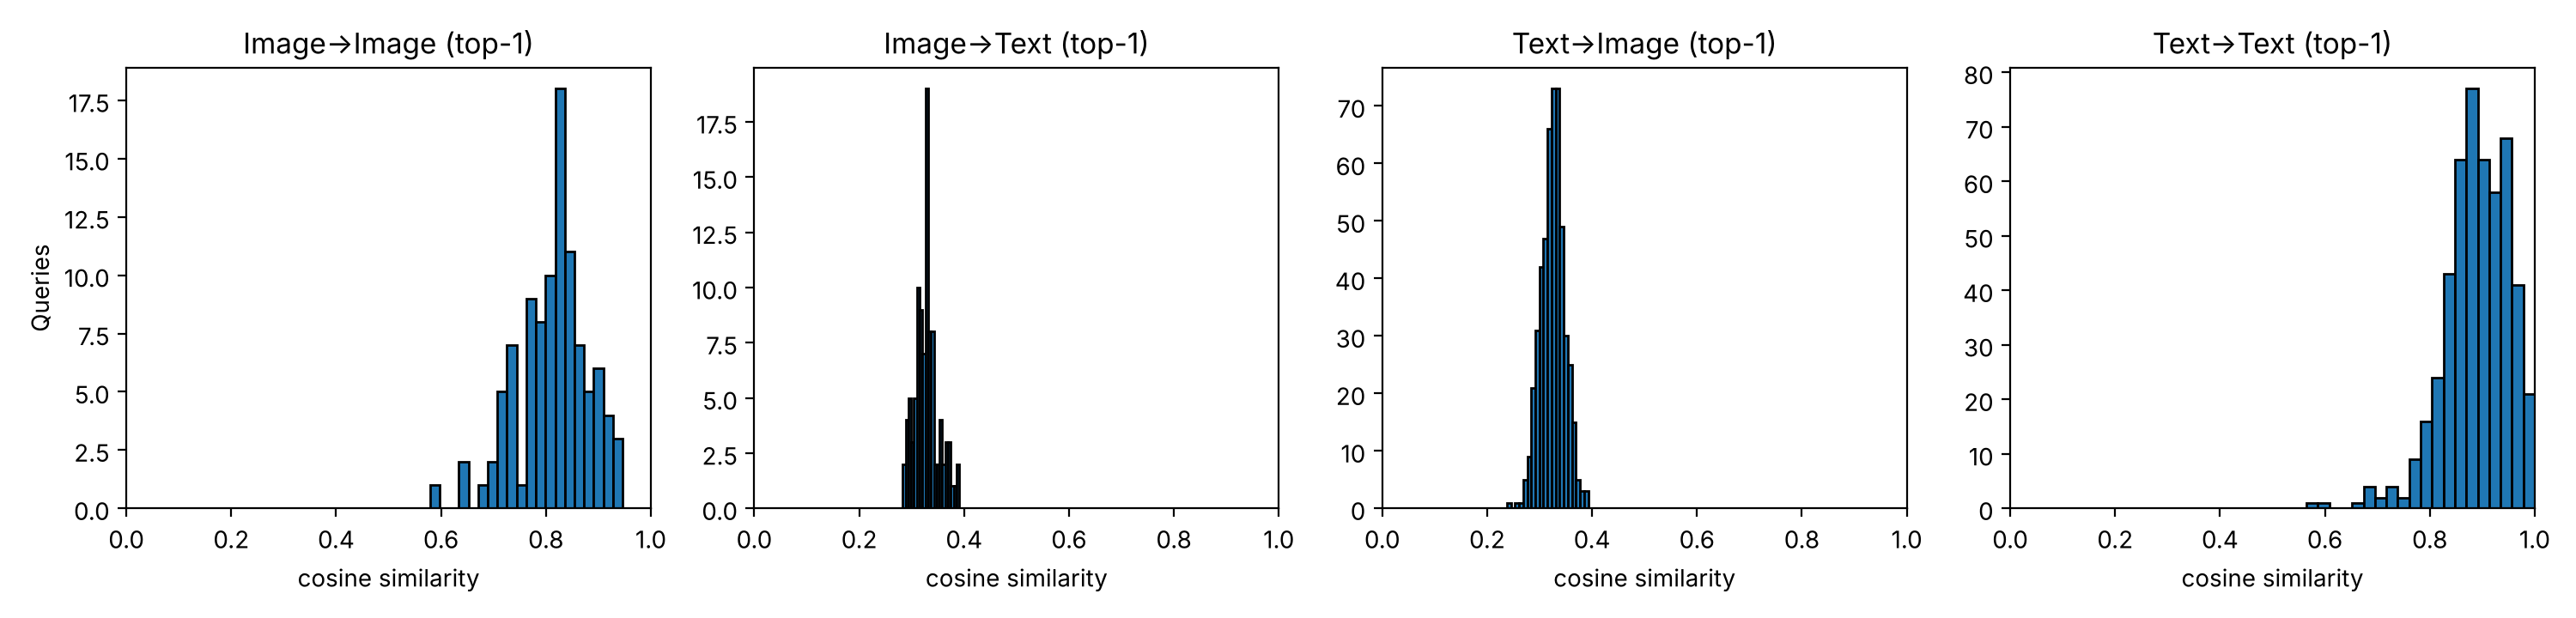
\includegraphics[width=\textwidth]{figures/retrieval_similarity.png}
\caption{Distribution of the top-1 cosine similarity for the four retrieval directions.}
\label{fig:retr}
\end{figure}

Additional observations: the 10th image neighbour has a mean similarity of 0.759 (vs. 0.814 for the first), 85 of the 500 text queries have a top-1 similarity $\ge 0.95$, and 9 reach exactly 1.0. For image-to-text, the ten retrieved captions come from 8.39 distinct images on average. Example: for the validation image 528231 (captions: ``Two black and white cows standing on a lush green field.'', \dots), the best image neighbour has a similarity of 0.946.

\begin{interp}
\begin{itemize}[nosep]
  \item \textbf{The pipeline works end to end.} Each query returns 10 results with valid IDs, and the scores are consistent with CLIP's behaviour, which confirms that embeddings, indexes and ID mappings are correctly linked.
  \item \textbf{Modality gap.} Same-modality similarities (I$\to$I $\approx0.81$, T$\to$T $\approx0.89$) are about 2.5 times larger than cross-modal ones (I$\leftrightarrow$T $\approx0.33$). This is the well-known \emph{modality gap} of CLIP: image and text embeddings occupy different regions of the sphere, and a cross-modal cosine of 0.3 is already a strong match. Consequently, \textbf{similarity thresholds must be chosen per modality} (the statement's thresholds 0.5, 0.7, 0.9 are meaningful for I$\to$I or T$\to$T, but would reject every cross-modal result), and scores from different directions must not be fused naively in hybrid RAG without normalisation.
  \item \textbf{Text-to-text exact matches.} The nine queries with similarity $1.0$ correspond to validation captions that are \emph{textually identical} (after lower-casing) to a caption in the knowledge base, e.g. ``A train traveling down tracks next to a forest.'' or ``A baseball player holding a bat during a game.'' This is not leakage (validation IDs are absent from the index), but a consequence of generic, repeated captions in COCO. It shows that text retrieval can return an identical sentence describing a \emph{different} image -- a reason to rely on image evidence as well and to treat caption similarity with caution.
  \item \textbf{Noise in the annotations.} One of the exact matches is the sentence ``There is no image here to provide a caption for.'', an annotator remark that is present in COCO. It confirms that a small amount of noisy captions exists in the data and could be retrieved as evidence.
  \item \textbf{Diversity of the retrieved captions.} The 8.39 distinct source images among 10 retrieved captions (image-to-text) show that retrieved captions mostly come from different images and are not dominated by the 5 captions of a single image, which is desirable for providing varied evidence.
\end{itemize}
\end{interp}


%====================================================================

\section{Validation and freezing of the release}

\subsection{Validation subset and selection of the pre-processing configuration}
The statement specifies that the 100 validation images are used to select the best pre-processing configuration before freezing. In this release, one pre-processing configuration is implemented (EXIF + RGB without resizing, minimal caption cleaning, CLIP ViT-B/32 with L2 normalisation, exact flat inner-product index). The validation subset was used to \emph{verify} that the pipeline works (Section~\ref{sec:retrieval}); no alternative configuration was compared on it. Alternatives that could be compared in the next phase on the same validation images are listed in Section~\ref{sec:limits}.

\subsection{Frozen artefacts}
\begin{table}[H]
\centering
\small
\renewcommand{\arraystretch}{1.15}
\begin{tabularx}{\textwidth}{@{}>{\raggedright\arraybackslash}p{6.3cm} >{\raggedright\arraybackslash}X@{}}
\toprule
\textbf{Frozen artefact} & \textbf{Content}\\
\midrule
{\footnotesize\code{data/splits/*.json}} & 10\,000 KB IDs, 100 validation IDs, 1\,000 test IDs (\code{test\_1000\_image\_ids.json}, seed 42) and the legacy 100-image test list.\\
{\footnotesize\code{data/captions/kb\_captions\_raw.json}} & 50\,028 raw captions (evaluation / generation context).\\
{\footnotesize\code{data/captions/kb\_captions\_cleaned.json}} & 50\,028 cleaned captions (retrieval and indexing only).\\
{\footnotesize\code{data/processed\_images/}} & 10\,000 RGB, EXIF-corrected images.\\
{\footnotesize\code{data/metadata/}} & Objects, bounding boxes, spatial relations per image; YOLO detections in \code{data/visual\_detections/} (merged file regenerated by \code{merge\_yolo\_metadata.py}).\\
{\footnotesize\code{data/embeddings/}} & $10\,000\times512$ image and $50\,028\times512$ text CLIP embeddings with ID arrays.\\
{\footnotesize\code{data/index/}} & FAISS \code{IndexFlatIP} image and text indexes with ID mappings.\\
{\footnotesize\code{reports/}} & Audit, exploration, pre-processing, QC and validation reports.\\
\bottomrule
\end{tabularx}
\caption{Frozen release shared with all groups.}
\label{tab:frozen}
\end{table}

\subsection{Freezing rules}
\begin{itemize}[nosep]
  \item No group may modify the test split or the knowledge base.
  \item Test reference captions must never be used during retrieval or generation; they are only used by the metrics.
  \item A test image must never be retrieved for itself: this holds because test images are not indexed.
  \item The raw captions are used for evaluation; cleaned captions only for retrieval.
\end{itemize}

%====================================================================

\section{Discussion and recommendations}
\label{sec:limits}

\subsection{Synthesis}
The data-preparation phase yields a coherent and verified base: complete raw data (no missing or corrupted file), a reproducible disjoint split (10\,000 / 100 / 100), a knowledge base of 10\,000 images and 50\,028 captions embedded with CLIP ViT-B/32 and indexed in exact FAISS indexes, and a quality-control report with 10/10 checks passed, including the leakage audit. The exploration shows that COCO is dominated by people in everyday scenes, with a strongly skewed number of objects per image, short and repetitive captions and a long-tailed object distribution; these properties will directly shape the retrieval and the hallucination analysis of the following phases.

\subsection{Limitations and deviations from the statement}
\begin{enumerate}[nosep]

  \item \textbf{No stratification} of the test subset: the 900 added images are drawn uniformly at random and the original 100 were random too, whereas the statement requires stratification (scene complexity, interactions, contexts).
  \item \textbf{Test-set size and audit}: the test set was extended from 100 to 1\,000 images, but \code{quality\_control.py} and \code{validate\_retrieval.py} (Table~\ref{tab:qc}, Section~\ref{sec:retrieval}) were run with the 100-image test file and have not been re-run.
  \item \textbf{Two exploration scopes}: object and caption statistics (Section~\ref{sec:explore}) are computed on the full train2017, while POS, colours, shapes and contexts are computed on the knowledge base (Section~\ref{sec:explore-kb}); the two scopes have not been unified.
  \item \textbf{Partial analyses}: colours and shapes come from captions (not pixels), indoor/outdoor and day/night from CLIP zero-shot (not verified labels); co-occurrences are exported as a table (top 20 pairs in the report) rather than a full matrix plot, and the spatial-relation distribution is not plotted.
  \item \textbf{Metadata}: the main metadata are COCO ground-truth annotations; YOLO detections (\code{yolo26n}, threshold 0.25) are provided as a realistic complement; object attributes are not annotated; spatial relations are coarse geometric relations computed from COCO boxes only.
  \item \textbf{Duplicates}: the 12 groups of identical images of train2017 are detected but not removed or cross-checked against the splits.
  \item \textbf{Indexing time} and \textbf{embedding-generation time} are printed by the scripts but not stored in a report file.
  \item \textbf{Single configuration}: only one pre-processing configuration was implemented, so no data-driven selection on the validation set was done.
  \item \textbf{CLIP centre-crop}: borders of landscape images are cropped at encoding time.
  \item \textbf{Retrieval validation without relevance labels}: only similarity scores are reported.
\end{enumerate}

\subsection{Recommendations for the next phases}
\begin{itemize}[nosep]
  \item Report the metrics per object-frequency band and per scene-complexity tercile to exploit the skew revealed by the exploration.
  \item Use modality-specific similarity thresholds and score normalisation (min--max or rank-based, e.g. reciprocal rank fusion) for hybrid RAG.
  \item Remove stop-words / rely on IDF for the BM25 index, given that 48.5\,\% of tokens are among 30 frequent words.
  \item Filter out noisy captions (such as ``There is no image here\dots'') or at least monitor their retrieval frequency.
  \item Define relevance labels from the COCO annotations (an image is relevant to a query if it shares the annotated objects) to compute Recall@k, Precision@k and MRR.
  \item Run \code{git lfs pull}, then re-run \code{explore\_knowledge\_base.py} and \code{extract\_metadata.py} if the exact knowledge-base totals (POS, colours, contexts, objects, relations) must be reported instead of values read from the figures.
\end{itemize}

%====================================================================
\section{Conclusion}
This first phase delivered the complete, documented and frozen data foundation of the project. The audit confirmed the integrity of COCO 2017 (no missing or corrupted image; 99.7\,\% of images with exactly five captions); the exploration characterised the data (80 object classes with ``person'' at 30.5\,\% of annotations, 7.27 objects and 10.48 words per caption on average); the eight pre-processing steps, completed by a YOLO detection branch and an extended 1\,000-image test set, produced a knowledge base of 10\,000 images and 50\,028 captions, embedded into a normalised 512-d CLIP space and indexed with exact FAISS inner-product indexes; and quality control (10/10 checks) together with a retrieval sanity test confirmed that the release is consistent, free of leakage and usable by all groups. 

%====================================================================
\begin{thebibliography}{9}
\bibitem{coco} T.-Y. Lin, M. Maire, S. Belongie, J. Hays, P. Perona, D. Ramanan, P. Doll\'ar and C. L. Zitnick, ``Microsoft COCO: Common Objects in Context'', in \emph{ECCV}, 2014.
\bibitem{clip} A. Radford, J. W. Kim, C. Hallacy, A. Ramesh, G. Goh, S. Agarwal, G. Sastry, A. Askell, P. Mishkin, J. Clark, G. Krueger and I. Sutskever, ``Learning Transferable Visual Models From Natural Language Supervision'', in \emph{ICML}, 2021.
\bibitem{faiss} J. Johnson, M. Douze and H. J\'egou, ``Billion-scale similarity search with GPUs'', \emph{IEEE Transactions on Big Data} 7(3), 2021.
\bibitem{rag} P. Lewis et al., ``Retrieval-Augmented Generation for Knowledge-Intensive NLP Tasks'', in \emph{NeurIPS}, vol.~33, 2020.
\end{thebibliography}

\end{document}

